\documentclass[eng,printmode,oneside]{mgr}
%opcje klasy dokumentu mgr.cls zostaly opisane w dolaczonej instrukcji

%ponizej deklaracje uzycia pakietow, usunac to co jest niepotrzebne
\usepackage{polski} %przydatne podczas skladania dokumentow w j. polskim
%\usepackage[polish]{babel}%alternatywnie do pakietu polski, wybrac jeden z nich
\usepackage[utf8]{inputenc} %kodowanie znakow, zalezne od systemu
\usepackage[T1]{fontenc} %poprawne skladanie polskich czcionek


%listingi
\usepackage{listings}
\usepackage{color}
\usepackage[usenames,dvipsnames]{xcolor}
%\usepackage{mathdots} 

\definecolor{zielony}{rgb}{0,0.6,0}
\definecolor{innyZielony}{rgb}{0.5,0.7,0}

\definecolor{mygreen}{rgb}{0,0.6,0}
\definecolor{mygray}{rgb}{0.5,0.5,0.5}
\definecolor{mymauve}{rgb}{0.58,0,0.82}
\definecolor{xmlString}{RGB}{200,16,0}
\definecolor{violet}{RGB}{80,33,97}
\definecolor{darkblue}{RGB}{15,1,255}
\definecolor{darkred}{RGB}{161,0,0}
\definecolor{greenJSP}{RGB}{25,154,12}
\definecolor{violetJSP}{RGB}{109,18,56}

\lstset{ %
  language=Java,
  backgroundcolor=\color{white},   % choose the background color; you must add \usepackage{color} or \usepackage{xcolor}
  basicstyle=\footnotesize,        % the size of the fonts that are used for the code
  breakatwhitespace=false,         % sets if automatic breaks should only happen at whitespace
  breaklines=true,                 % sets automatic line breaking
  captionpos=b,                    % sets the caption-position to bottom
  commentstyle=\color{mygray},    % comment style
  deletekeywords={...},            % if you want to delete keywords from the given language
  extendedchars=true,              % lets you use non-ASCII characters; for 8-bits encodings only, does not work with UTF-8
  frame=single,                    % adds a frame around the code
  keepspaces=true,                 % keeps spaces in text, useful for keeping indentation of code (possibly needs columns=flexible)
  keywordstyle=\color{darkred}\textbf,       % keyword style
  morekeywords={},            % if you want to add more keywords to the set
  numbers=left,                    % where to put the line-numbers; possible values are (none, left, right)
  numbersep=5pt,                   % how far the line-numbers are from the code
  numberstyle=\tiny\color{mygray}, % the style that is used for the line-numbers
  rulecolor=\color{black},         % if not set, the frame-color may be changed on line-breaks within not-black text 
  showspaces=false,                % show spaces everywhere adding particular underscores; it overrides 'showstringspaces'
  showstringspaces=false,          % underline spaces within strings only
  showtabs=false,                  % show tabs within strings adding particular underscores
  stepnumber=1,                    % the step between two line-numbers. If it's
  % 1, each line will be numbered
  stringstyle=\color{blue},     % string literal style
  tabsize=2,                       % sets default tabsize to 2 spaces
  %identifierstyle=\color{blue},
  %title=\lstname,                   % show the filename of files included with
  % \lstinputlisting; also try caption instead of title
  keywordstyle=[3]{\color{darkblue!50!black}},
  keywordstyle=[4]{\color{greenJSP!50!black}\textbf},
  keywordstyle=[5]{\color{violetJSP!50!black}\textbf},
  escapeinside={(*@}{@*)}
}
\newcommand{\CodeSymbol}[1]{\textcolor{greenJSP}{#1}\textbf}

\usepackage{url}

%kolor do komentarzy, uwag, przypomnienie
\definecolor{komentarz}{rgb}{1,0,0}
 
%pakiety do grafiki
\usepackage{graphicx}
\usepackage{subfigure}
%\usepackage{psfrag}
\usepackage[justification=centering]{caption}
\usepackage{wrapfig}
%\usepackage{lipsum}
%\usepackage{subcaption}

%pakiety dodajace duzo dodatkowych polecen matematycznych
\usepackage{amsmath} 
\usepackage{amsfonts}

%pakiety wspomagajace i poprawiajace skladanie tabel
\usepackage{supertabular}
\usepackage{array}
\usepackage{tabularx}
\usepackage{hhline}

%pakiet wypisujacy na marginesie etykiety rownan i rysunkow zdefiniowanych przez \label{}, 
%schcac wygenerowac finalna wersje dokumentu wystarczy usunac 
%ponizsza linie
%\usepackage{showlabels}
\sloppy

%definicje wlasnych polecen
\newcommand{\R}{I\!\!R} %symbol liczb rzeczywistych, dziala tylko w trybie matematycznym
\newtheorem{theorem}{Twierdzenie}[section] %nowe otoczenie do skladania twierdzen

%dane do zlozenia strony tytulowej
\title{System monitoringu lokalizacji przesyłek kurierskich}
\engtitle{English title}
\author{Monika Strachowska}
\supervisor{Prof dr hab. inz. Czesław Smutnicki, \newline Katedra \ldots}
%\guardian{dr hab. inz. Imie Nazwisko Prof. PWr, I-6} %nie uzywac jesli opiekun jest ta sama osoba co prowadzacy prace

%\date{2008} %standardowo u dolu strony tytulowej umieszczany jest biezacy rok, to polecenie pozwala wstawic dowolny rok

%ponizej jest lista kierunkow i specjalnosci na wydziale elektroniki, nalezy wybrac wlasciwe lub dopisac jesli nie ma odpowiednich
\field{Automatyka i Robotyka (AIR)}
\specialisation{Systemy informatyczne w automatyce (ASI)}

%tutaj zaczyna sie wlasciwa tresc dokumentu
\begin{document}

\bibliographystyle{plabbrv} %tylko gdy uzywamy BibTeXa, ustawia polski styl bibliografii

\maketitle %polecenie generujace strone tytulowa


\tableofcontents %spis tresci

%ponizej znajduje sie przykladowa tresc dalszej czesci dokumentu, zainteresowanych zachecam do rozszyfrowania frazy "Lorem ipsum" :)
\chapter{Wstęp i cel pracy}

Współcześnie coraz więcej osób korzysta z możliwości zakupów przez internet, co
niesie za sobą wiele korzyści. Często zakupiony towar jest tańszy, unikalny,
bądź niedostępny w stacjonarnym sklepie czy po prostu jest to wygodniejsza forma
zakupów. Konieczność dostarczenia przedmiotów nabytych w ten sposób skutkuje
szybszym rozwojem usług w zakresie transportu. Oprócz wyżej wymienionych zakupów
istotną rolę w branży transportowej pełnią dokumenty, które nierzadko muszą być
dostarczone jak najszybciej.
Oczywistym jest, że ludzie zamawiający usługi kurierskie chcieliby otrzymać
usługę o jak najwyższej jakości. Zwiększenie jakości tej usługi może nastąpić poprzez
skrócenie czasu dostarczenia przesyłki (co fizycznie już jest bardzo trudne),
niższy jej koszt, czy na przykład możliwość sprawdzenia, w jakim dokładnie
miejscu ona się znajduje. Dokładna lokalizacja przesyłki -- taka funkcjonalność
usługi kurierskiej nie należy do jakości wymaganej i koniecznej, ale znacznie podniesie prestiż firmy
kurierskiej, która zdecyduje się na takie dodatkowe udogodnienie. Klient może
czuć się bardziej komfortowo wiedząc gdzie jest przesyłka, dzięki czemu może
zaplanować sobie dzień, w którym nastąpi dostawa.

Przedstawiany tu projekt rozwija funkcjonalność firm kurierskich o
graficzne przedstawienie (w formie mapy) aktualnej lokalizacji przesyłki
poprzez lokalizowanie kuriera, który w danym momencie posiada ją
w swoim samochodzie .
Taka forma prezentacji jest prosta w odbiorze i bardziej czytelna niż wyniki
jakie prezentowane są aktualnie w formie tabel, w których zawarte są miejsca
zeskanowania przesyłki. Ponadto praca próbuje rozwiązać problem jaki istnieje w
estymacji czasu dostarczaniu przesyłki do adresata; obecnie estymacja czasu
dostarczenia jest bardzo niedokładna (ogólna) lub w ogóle jej nie ma.

W niniejszej pracy został przedstawiony zrealizowany system lokalizacji
przesyłek kurierskich. System składa się z aplikacji kurierskiej
zaprojektowanej na platformę Android. Aplikacja wysyła na serwer lokalizację
kuriera odczytaną z czujników GPS. Odczyt ten jest przetwarzany przez serwer i
zapisywany do bazy danych. Serwer po otrzymaniu pozycji kuriera oraz wiedzy jaką
paczkę w danej chwili posiada przy sobie kurier, może bezbłędnie określić
lokalizację każdej przesyłki zarejestrowanej w systemie.
Drugą składową systemu jest serwis kliencki, który umożliwia sprawdzenie pozycji
przesyłki oraz dodanie nowego zlecenia.

W rozdziale drugim opisano wykorzystane w projekcie technologie, są to między
innymi język Java, Servlet, baza danych, system Android. W kolejnym, trzecim
rozdziale opisano jak działa zaprojektowany system oraz z czego się składa.
W rozdziale przedstawiono główne, kluczowe dla działania systemu metody klas,
widok graficzny aplikacji mobilnej i serwisu oraz diagram bazy danych.
Kolejny rozdział pokrótce przedstawia jak należy przygotować środowisko do pracy z takim systemem.

\chapter{Wykorzystane technologie}

Zrealizowany projekt bazuje na nowoczesnych technologiach.
Wykorzystano urządzenie mobilne -- telefon komórkowy z systemem
Android, bazę danych do przechowywania informacji, a także serwer, który to
łączy wszystkie elementy w spójną całość. Głównym językiem
programowania użytym w projekcie jest język Java, dzięki któremu
zrealizowano aplikację mobilną, obsługę Servletu, bazy danych, odpytywania i
parsowania odpowiedzi serwera Google o odległości pomiędzy dwoma wskazanymi
punktami, a także obsługa witryny zapytań z aplikacji webowej. Kompletny system
powstał przy użyciu IDE Eclipse z odpowiednimi dodatkami.

\section{Java}

Java jest obiektowym językiem programowania ogólnego przeznaczenia.
Charakteryzuje się silnym ukierunkowaniem na obiektowość oraz niezależnością od
architektury sprzętowej i przenośnością aplikacji pomiędzy platformami.
Oprócz wyżej wymieniowych założeniami języka Java jest prostota, sieciowość,
niezawodność, bezpieczeństwo, interpretowalność, wysoka wydajność czy możliwość
programowania współbieżnego.

Java to język:

\begin{itemize}
  \item  \parbox[t]{\dimexpr\textwidth-\leftmargin}{
      \vspace{-2.5mm}
    \begin{wrapfigure}{R}{0.3\textwidth}
	\centering
	
\includegraphics[width=0.18\textwidth]{javaEE.png}
	\caption{\label{fig:javaEE}Logo Java EE \cite{java.oracle.ee}}
	\end{wrapfigure}
  Prosty -- założeniami autorów języka Java było, aby programista bez
  specjalnych szkoleń mógł od razu zacząć pisać proste aplikacje. Składnia
  została uproszczona (w stosunku do C++) o arytmetykę wskaźnikową, struktury,
  unie, przeciążanie operatorów itd. 
	}
  \item Zorientowany obiektowo;
  \item Sieciowy --- posiada wbudowaną bibliotekę, która w przystępny sposób
  umożliwia pracę z protokołami HTTP, TCP/IP, FTP;
  \item Niezawodny --- szczególnie skupiono się na wykrywaniu ewentualnych
  błędów w czasie kompilacji, zapobieganiu sytuacjom, w których błąd może
  wystąpić oraz obsłudze błędów w czasie działania programu;
  \item Bezpieczny --- w związku z naciskiem położonym na zastosowania sieciowe
  zadbano o możliwie najlepsze zabezpieczenie przed wirusami i ingerencją osób
  trzecich;
  \item Niezależny od architektury --- kod źródłowy kompilowany jest do kodu
  pośredniego (bajtowego), który następnie jest interpretowany na maszynie
  wirtualnej Javy(JVM), dostosowanej do odpowiedniego systemu i platformy sprzętowej. Maszyna
  wirtualna Javy jest zdolna wykonywać program z kodu pośredniego. Z tego powodu język Java
  stosowany jest na wielu urządzeniach oraz różnych systemach operacyjnych.
  Niestety konsekwencją przenośności kodu może być jego suboptymalna
  wydajność, a w konsekwencji wolniejsze działanie;
  \item Przenośny --- posiada ściśle określone rozmiary typów danych i nie ma
  możliwości zmiany ich rozmiaru przez programistę czy np.
  zmiana kolejności bitów;
  \item Interpretowany --- program nie jest kompilowany tylko przechowywany w
  postaci kodu bajtowego, podczas uruchomienia zostaje dopiero interpretowany i
  uruchamiany przez interpreter języka;
  \item Elastyczny --- istnieje możliwość tłumaczenia kodu bajtowego w locie,
  co zwiększa szybkość ładowania się programu;
  \item Wielowątkowy --- umożliwia przetwarzanie współbieżne z wykorzystaniem
  wątków, a także pracę w czasie rzeczywistym;
  \item Dynamiczny --- obiekty w Javie można zmieniać w zależności od
  zmieniającego się środowiska, możliwy jest wgląd we wszystkie obiekty i
  rozszerzenie je o nowe metody;
\end{itemize}

Język Java wywodzi się z języków C++ i C. Wykorzystuje wiele potrzebnych i
użytecznych funkcji tych języków, a z mniej użytecznych, trudnych w
implementacji lub często powodujących błędy -- zrezygnowano. Język Java
umożliwia dziedziczenie, a ponadto wszystkie obiekty Javy są podklasą obiektu
bazowego. Jednakże Java nie umożliwia dziedziczenia wielobazowego, dlatego wprowadzono interfejsy -
abstrakcyjny typ, który definiuje jedynie metody bez implementacji i nie
posiada stanu. Z tego powodu można jedynie implementować
interfejs lub wykorzystać go do utworzenia klas anonimowych. Język Java
umożliwia pisanie aplikacji stacjonarnych, webowych czy mobilnych. Duży nacisk
położono na zaprojektowanie systemu wyjątków. Zbieraniem i ponownym
korzystaniem z zasobów po obiektach bez referencji (nie wykorzystywanych -- bez
odwołania w kodzie) zajmuje się wbudowany \texttt{GarbageCollector} (kolektor
nieużytków) \cite{java.doc}.

\section{Wzorzec architektoniczny -- MVC}

W projekcie do zorganizowania struktury aplikacji serwerowej został zastosowany
wzorzec architektoniczny MVC (Model-View-Controller). W modelu tym Model jest
odpowiedzialny za przechowywanie logiki, z której korzystają inne składowe
systemu. Kolejną częścią składową tej struktury jest Widok, który to jest
\makebox[\linewidth][s]{odpowiedzialny za funkcje prezentacji
w ramach interfejsu użytkownika, ale także może posiadać} swoją
logikę. Ostatnim elementem systemu jest Kontroler, który spaja dwie wcześniejsze
części. Kontroler odpowiada za przepływ danych od/do użytkownika, reakcję
systemu w zależności od zachowania użytkownika -- zarządza
takzę Modelem i Widokiem. W takiej strukturze jest jasno zdefiniowane, która
część systemu pełni jakie funkcje. Ta struktura architektoniczna 
jest najczęściej stosowana w aplikacjach WWW, gdzie widać
wyraźną granicę pomiędzy widokiem i modelem, a kontrolerem jest serwer, który
obsługuje informacje płynące z widoku (z HTTP), odpowiednio formuje model i
przekazuje go do widoku \cite{java.mvc,java.mvc.grafika}.

\begin{figure}[ht!]
\centering
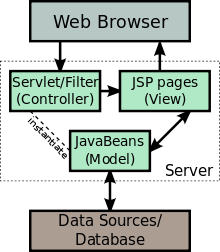
\includegraphics[width=60mm]{jspModel.png}
\caption{Schemat systemu zaprojektowanego według wzorca
Model-View-Controller model 2 \cite{java.mvc.grafika}}
\label{fig:MVC2}
\end{figure}

Autor w swojej pracy użył modelu MVC2 [rys. \ref{fig:MVC2}]
Uzasadnieniem użycia tego wzorca jest ułatwiona organizacja aplikacji, w której
istnieje interfejs graficzny użytkownika. Dzięki niemu w prosty i logiczny
sposób można było rozdzielić logikę, kontrolę i reprezentację. Kontrolerem z
rysunku \ref{fig:MVC2} jest opisany w kolejnym podrozdziale Servlet.

\newpage
\section{Servlet}

Serwlety to aplikacje działające na serwerze WWW napisane w języku Java, mające
zapewnić działanie aplikacji internetowych niezależnie od platformy.
Umożliwiają korzystanie z baz danych i obsługę żądań i odpowiedzi HTTP. Z tego
powodu wykorzystywane są do budowania interaktywnych aplikacji internetowych.

\begin{wrapfigure}{r}{0.3\textwidth}
\centering
\subfigure {

\includegraphics[width=10ex]{feather.png}

\includegraphics[width=10ex]{tomcat.png}
}
\caption{\label{fig:apache}Logo Apache i Apache Tomcat \cite{apache.org,tomcat.org}}
\end{wrapfigure}

Serwer Apache obsługuje komunikację z klientem za pomocą protokołu HTTP. Wybrana
w projekcie dystrybucja Tomcat Apache [rys. \ref{fig:apache}] jest projektem o
otwartym kodzie źródłowym. Wykorzystuje wielowątkowość, jest skalowalny i
bezpieczny oraz zapewnia kontrolę dostępu \cite{apache.org}.

Wybór Tomcat Apache na serwer podyktowany był przez wybór Javy jako głównego
języka projektu. Serwlet jest dość popularnym narzędziem, co pomogło także w
uruchomieniu i skonfigurowaniu go.

\section{JavaServer Pages}

JSP (ang. JavaServer Pages) jest to technologia, dzięki której możliwe jest
dynamiczne tworzenie stron internetowych. JSP bazuje na językach znaczników,
np.
HTML, XML oraz innych. Technologia ta jest kompatybilna z Serwletami (Apache
Tomcat i innymi).

To właśnie wprowadzenie plików JSP wymaga korzystania z wcześniej
opisanego modelu MVC [rys. \ref{fig:MVC2}]. W dodatku JSP oprócz użycia języków
znaczników umożliwia przeplatanie ich z językiem Java. Wtedy kod, który będzie
napisany w Javie musi być ujęty w znaki <\% \ldots \%>, np. fragment z listingu
\ref{lst:Sprawdz.jsp}:

\texttt{<\% out.print("Nadawca"); \%> \$\{regUserName\}
\$\{regUserAddr\}}

Natomiast frazy ujęte w znaki \$\{\ldots\} służą do dostępu (pobrania
i/lub wysyłania) do argumentów i funkcji, które powstały w obiektach Javy. Żeby
przekazać taką wartość z klasy Javy, klasa ta musi rozszerzać klasę Servlet
(\texttt{extends HttpServlet}) oraz ustawiać parametr o nazwie jak w pliku *.jsp
\{\} dodając go do kontekstu \texttt{HttpServletRequest}; jako przykład podano
fragment z listingu \ref{lst:Sprawdz.doPost.java}:

\texttt{req.setAttribute("regUserName",
						searchParcel.getRegisteredUserNameUser());}

\section{Technologie internetowe}

W przedstawionym w tej pracy projekcie korzystano z technologi internetowych,
które zapewniały interakcję z użytkownikiem oraz obsługę stron WWW. Skorzystano
z takich technologii jak:
\begin{itemize}
  \item JavaScript --- skryptowy język programowania stosowany głównie do
  tworzenia stron internetowych, zapewnia interakcję z
  użytkownikiem \cite{javascript.dev}, służy do kontroli przeglądarki, zmiany
  treści strony. Składnia języka JavaScript jest zbudowana na podstawie języka
  C. Język ten charakteryzuje się dynamicznym systemem typów oraz obiektowością;
  \item HTML --- język znaczników służący do tworzenia stron
  internetowych. Język ten składa się z tagów umieszczonych w
  nawiasach trójkątnych (\texttt{<\ldots>}), które mogą zawierać inne
  elementy HTML. Napisy umieszczane są pomiędzy tagami \texttt{<tag> napis
  </tag>}, gdzie pierwszy znacznik jest tagiem oznaczającym początek, a drugi -- zamykającym.
  HTML jest budulcem strony internetowej opisującym jej strukturę.
  Można go osadzać w takich językach jak JavaScript, a do definiowania wyglądu i
  układu tekstu i innych elementów na stronie można użyć stylów CSS;
  \item XML --- język znaczników przeznaczony do reprezentowania danych w
  strukturyzowany sposób \cite{xml.wiki}. Tak jak HTML składa się ze znaczników
  \texttt{<\ldots>} i \texttt{</\ldots>} lub samozamykających
  \texttt{<\ldots/>}.
  \item Protokół HTTP --- podstawy protokół komunikacji w internecie służący
  do wymiany informacji. Funkcjonuje w trybie żądanie-odpowiedź w modelu
  klient-serwer, gdzie przykładowo przeglądarka jest klientem, a aplikacja
  uruchomiona na komputerze -- serwerem. HTTP jest protokołem warstwy aplikacji,
  która zapewnia komunikację.
\end{itemize}

\newpage
\section{Baza Danych -- MySQL}

W projekcie do przechowywania danych skorzystano z baz danych. Baza danych
pozwala w ustrukturyzowany sposób kolekcjonować dane niezbędne do działania
programów. Przechowywane dane mogą być w dowolnym formacie i strukturze.

\begin{wrapfigure}{r}{0.3\textwidth}
\centering

\includegraphics[width=0.2\textwidth]{logomysql.png}
\caption{Logo MySQL \cite{Mysql.com}}
\label{fig:mysql}
%\vspace{-10pt}
\end{wrapfigure}

Systemem bazodanowym wykorzystanym w projekcie był MySQL rozwijany przez
firmę Oracle. Jest to rozwiązanie o otwartym kodzie źródłowym do zarządzania
relacyjnymi bazami danych.
Charakteryzuje się takimi cechami jak szybki, wielowątkowy dostęp z możliwością
obsłużenia dużej ilości użytkowników. Serwer MySQL może być stosowany do
systemów, w których znajdują się dane o znaczeniu krytycznym lub te systemy są
mocno obciążane \cite{Mysql.com}.

Język MySQL posiada takie typy danych jak signed/unsigned int, long, float,
double, char, varchar, date, time, datetime, enum i inne. Język MySQL składa się
z takich typów komend jak: DML (ang.
Data Manipulation Language -- dotyczące manipulowania), DLL (ang. Data
Defitnition Language) oraz DCL (ang. Data Control Language).
Komendy DML:
\begin{itemize}
  \item \texttt{select} --- służy do otrzymywania wierszy z wybranych tabeli,
  najpopularniejsza forma użycia komendy \texttt{select}:
    
  \texttt{SELECT select\_expr [, select\_expr] [FROM table\_name] [WHERE
  where\_condition];}
  
  \item \texttt{insert} --- komenda ta wstawia nowe wiersze do istniejącej tabeli,
  istnieją trzy przypadki użycia tej komendy:
  
  \texttt{INSERT [INTO] table\_name [(col\_name,...)]
    {VALUES | VALUE} ({expr | DEFAULT},...),\newline (...), ...
    [ ON DUPLICATE KEY UPDATE
      col\_name=expr
        [, col\_name=expr] ... ];} 
  
  \texttt{INSERT [INTO] table\_name SET col\_name={expr | DEFAULT}, ... [ ON
  DUPLICATE KEY \newline UPDATE col\_name=expr [, col\_name=expr] ... ];}
      
   \texttt{INSERT [INTO] table\_name [(col\_name,...)]
    SELECT ... \newline[ ON DUPLICATE KEY UPDATE
      col\_name=expr
        [, col\_name=expr] ... ];}
  
  \item \texttt{update} --- aktualizuje kolumny istniejących wierszy,
  struktura użycia komendy:
  
  \texttt{UPDATE table\_name
    SET col\_name1={expr1|DEFAULT} [, col\_name2={expr2|DEFAULT}] ...
    \newline[WHERE where\_condition];}
  
  \item \texttt{delete} --- usuwa pojedyncze wiersze, użycie komendy:
  
  \texttt{DELETE FROM table\_name [WHERE where\_condition];}
  
  \item i inne
\end{itemize}
Komendy DLL:
\begin{itemize}
  \item \texttt{create} --- komenda stosowana w połączeniu z database, function,
  index, procedure, table, trigger, view. Komenda używana jest do
  dodawania nowej bazy danych czy tabeli;
  \item \texttt{alter} --- komenda używana w połączeniu z database, table,
  function, procedure oraz view. Służy do zmiany struktury bazy danych, tabeli,
  itp., np. można dodać lub usunąć kolumnę istniejącej tabeli;
  \item \texttt{drop} --- umożliwia usunięcie bazy danych i tabeli.
\end{itemize}
Komendy DML:
\begin{itemize}
  \item \texttt{commit} --- zatwierdza wpisaną transakcję, wprowadzona zmiana jest
  permanentna;
  \item \texttt{rollback} --- wycofuje ostatnią wpisaną transakcję.
\end{itemize}

Oprócz wyżej wymienionych MySQL posiada również inne komendy, jednak są one
znacznie rzadziej wykorzystywane, dlatego nie zostały tutaj przytoczone.

\newpage
\section{Android}

Android jest systemem operacyjnym wykorzystywanym na platformach mobilnych,
zbudowanym w oparciu o jądro Linux. Umożliwia tworzenie aplikacji na wiele
urządzeń -- dokonywane to jest przez dostowanie pliku XML, w którym
dostosowuje się aplikację do konkretnej wersji API. System Android ma taką
właściwość, że każda włączona aplikacja jest uruchamiana na maszynie
wirtualnej i jest niezależna od pozostałych. Najnowszą wersją systemu
jest Lollipop 5.0.

Rozpoczęcie pracy deweloperskiej z Androidem zaczyna się od instalacji
środowiska --- Eclipse z dodatkiem SDK Android lub Android Studio. Po
zainstalowaniu IDE projektowanie aplikacji zaczyna się od opracowania układu
interfejsu użytkownika, następnie przechodzi się do oprogramowania
funkcjonalności oraz logiki aplikacji. Po zakończeniu etapu budowania aplikacji
następuje testowanie jej \cite{developer.android}.

System Android składa się z czterech podstawowych elementów:

\vspace{-2mm}
\begin{itemize}
  \item \parbox[t]{\dimexpr\textwidth-\leftmargin}{
     \vspace{-2.5mm}
    \begin{wrapfigure}{R}{0.22\textwidth}
	\centering
	
\includegraphics[width=0.1\textwidth]{andlogo.png}
	\caption{\label{fig:andlogo}Logo systemu Android \cite{developer.android}}
	\end{wrapfigure}
  Activity --- reprezentuje ekran użytkownika, przykładem jest aplikacja
  do obsługi emaila, która posiada jedną aktywność do listowania nowych
  wiadomości i inną do pisania ich. Aktywności implementuje się używając
  podklasę \texttt{Activity};
  \item Service --- jest to składnik aplikacji, usługa, która działa w tle.
  Przykładem takiej usługi \texttt{Services} może być odtwarzacz muzyki, który
  jest uruchomiony w tle i w tym samym czasie użytkownik może korzystać z innych aplikacji w urządzeniu.
  Taką własność aplikacji implementuje się za pomocą podklasy \texttt{Service};
	}
  \item Content provider --- służy do zarządzania wspólnymi danymi, a także
  danymi, które są prywatne dla danej aplikacji. Zarządzanie danymi
  implementuje się stosując podklasę \texttt{ContentProvider};
  \item Broadcast receiver --- komponent systemu, który jest
  odpowiedzialny za rozgłaszanie informacji w systemie, np. informacja o
  niskim stanie baterii jest wyświetlana niezależnie od aktywności w urządzeniu.
  Taką cechę aplikacji uzyskuje się implementując podklasę \texttt{BroadcastReceiver}.
\end{itemize}

Aplikacja w systemie Android składa się z wielu części, które są ze
sobą luźno powiązane. Zazwyczaj jedna część aplikacji jest główna -- najczęściej
ta, która jest pokazywana użytkownikowi po uruchomieniu aplikacji.
Następnie każde działanie wykonane na tym ekranie może uruchamiać inny ekran,
proces czy działanie. Wtedy przy każdym uruchomieniu nowej działalności
wcześniejsza jest zatrzymywana i przechowywana na stosie -- LIFO (ang. last in
first out). Dzięki temu użytkownik ma możliwość wrócić do poprzedniej
działalności (ekranu) cofając się, wtedy zdejmowana jest ona ze stosu w takim
stanie w jakim była pozostawiona.

Wart uwagi jest element \texttt{Activity}, reprezentujący ekran użytkownika,
oferujący interakcję z użytkownikiem. Najczęściej okno aplikacji wypełnia
cały wyświetlacz, ale może być mniejsze lub pływające na tle innych okien.

Utworzenie aplikacji korzystającej z właśności \texttt{Activity} wymaga
zaimplementowania podklasy \texttt{Activity}, w tej podklasie należy zdefiniować metody, które będą
określały aktywność pomiędzy różnymi stanami cyklu jej życia. Przez cykl życia
aktywaności rozumie się jej tworzenie, zatrzymywanie, wznawianie i niszczenie.
Metoda \texttt{onCreate()} określa stan aktywności podczas jej tworzenia. Metoda
\texttt{onPause()} definiuje stan aktywności w momencie opuszczenia jej przez
użytkownika. Opuszczenie aktywności nie musi oznaczać jej zakończenia, typowo
zachowywany jest aktualny stan.

Z powyższego da się zauważyć, że istotną kwestią jest zarządzanie życiem
aktywności. Aktywność może być zatem w jednym z trzech stanów: wznowiona, 
wstrzymana oraz zatrzymana. Stan wznawiania określa stan, w którym aplikacja
jest włączona i znajduje się na głównym planie ekranu użytkownika. Stan
wstrzymania dotyczy stanu, w którym aplikacja jest widoczna (włączona), jednak
nie znajduje się na głównym ekranie. Stan zatrzymania oznacza, że aplikacja jest
całkowicie przysłonięta przez inne i pracuje w tle. W stanie wstrzymania i
zatrzymania system, w przypadku braku pamięci, może zatrzymać aplikację.

Na rysunku \ref{fig:andActivityLifecycle} przedstawiony został cykl życia
aktywności. Wspomniana metoda \texttt{onCreate()} wywoływana jest zawsze wtedy,
gdy aplikacja jest uruchamiana po raz pierwszy, w tym miejscu tworzone są widoki.
Następną wywoływaną metodą jest \texttt{onStart()}, która wywołuje pokazanie się
aplikacji pod restarcie lub zatrzymaniu aplikacji. Metoda \texttt{onResume()} wywoływana jest
zawsze po pauzie i rozpoczyna interakcję z użytkownikiem, odpowiada za
przywołanie aktywności na szczyt stosu. \texttt{onPause()} wywoływana jest w
momencie wstrzymywania aktualnej aktywności. Metoda \texttt{onStop()} zostaje
wykonana, gdy aplikacja ma przejść w stan niewidoczny dla użytkownika -- po
wywołaniu tej metody aktywność może zostać zniszczona, zamknięta lub
zrestartowana.
Ostatnią metodą przed zniszczeniem aktywności jest \texttt{onDestroy()} -- zamyka
wszystkie otwarte procesy.

\begin{figure}[ht!]
\centering
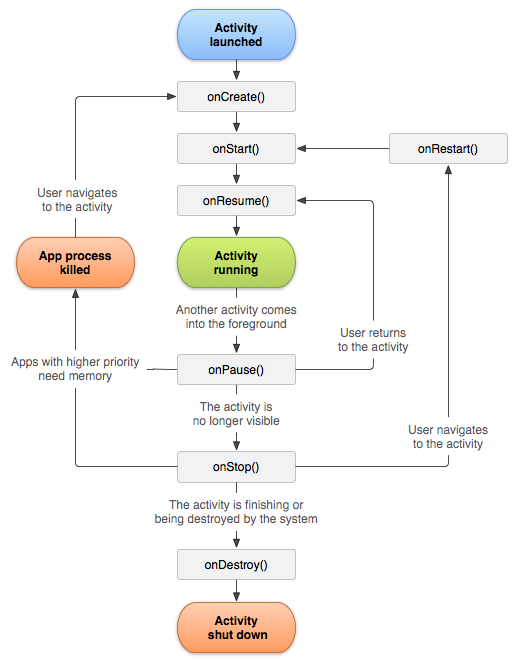
\includegraphics[width=80ex]{andActivityLifecycle.png}
\caption{Cykl życia aktywności w systemie Android \cite{developer.android}}
\label{fig:andActivityLifecycle}
\end{figure}

\section{Google Maps API}

Firma Google udostępnia korzystanie deweloperom ze swoich produktów
\cite{developer.google}. W projekcie autor korzysta z Google Maps API. Google
Maps jest to zbiór interfejsów HTTP usług Google do stosowania w połączeniu z
mapą. Wysłanie zapytania HTTP o określonym formacie URL o położenie, trasę czy
odległość pomiędzy punktami generuje odpowiedź po stronie serwera. Po zapytaniu
odpowiedź dostarczana jest w formacie JSON lub XML. W projekcie autor korzystał z dwóch
usług Google Maps API -- jedną była \texttt{Google Maps JavaScript API v3
Directions Service}, drugą \texttt{Distance Matrix API}.

\begin{wrapfigure}{r}{0.3\textwidth}
\centering
\vspace{-15pt}

\includegraphics[width=0.3\textwidth]{googlelogo.png}
\caption{Logo Google Developers \cite{developer.google}}
\label{fig:googlelogo}
\vspace{-10pt}
\end{wrapfigure}

\texttt{Google Maps JavaScript API v3} jest usługą Google, która oblicza trasę
pomiędzy dwoma punktami za pomocą obiektu \texttt{DirectionsService}.
Wspomniany obiekt łączy się z serwisem \texttt{Google Maps API} i pobiera od niego wynik, uwzględniając wskazówki
dotyczących obliczenia trasy. Do wyrysowania mapy i
trasy z uzyskanej odpowiedzi \texttt{DirectionsService} korzysta się z
\texttt{DirectionsRenderer}. Zapytanie \texttt{JavaScript API V3 Directions
Service} jest wykonane w języku JavaScript.

Na listingu \ref{lst:DirectionsRequest} przedstawione zostały wszystkie możliwe
parametry jakie może przyjmować obiekt \texttt{DirectionsRequest}. Oczywiście
większość tych parametrów jest opcjonalna, wymagane są jedynie \texttt{origin},
\texttt{destination} i \texttt{travelMode}.

\lstset{language=Java,firstnumber=1,stepnumber=1,keywords=[5]{String,
LatLng,TravelMode,TransitOptions,UnitSystem,Boolean,DirectionsWaypoint}} 
\begin{lstlisting}[caption=Parametry jakie może
przyjmować obiekt typu \texttt{DirectionsRequest},label=lst:DirectionsRequest] 
{
  origin: LatLng | String,
  destination: LatLng | String,
  travelMode: TravelMode,
  transitOptions: TransitOptions,
  unitSystem: UnitSystem,
  durationInTraffic: Boolean,
  waypoints[]: DirectionsWaypoint,
  optimizeWaypoints: Boolean,
  provideRouteAlternatives: Boolean,
  avoidHighways: Boolean,
  avoidTolls: Boolean
  region: String
}
\end{lstlisting}

Na powyższym listingu przedstawione parametry oznaczają:
\begin{itemize}
  \item \texttt{origin} --- punkt startowy;
  \item \texttt{destination} --- punkt końcowy;
  \item \texttt{travelMode} --- rodzaj transportu: pojazd, rower, tranzyt, na
  pieszo;
  \item \texttt{transitOptions} --- określa, czy wynik zapytania powinien zawierać
  informację o natężeniu ruchu;
  \item \texttt{unitSystem} --- określa w jakich jednostkach ma być wyświetlany
  dla użytkownika wynik: jednostki metryczne lub jednostki imperialne;
  \item \texttt{durationInTraffic} --- wynik zawiera czas podróży przy aktualnym
  natężeniu ruchu;
  \item \texttt{waypoints[ ]} --- punkty pośrednie trasy
  \item \texttt{optimizeWaypoints} --- optymalizuje trasę na podstawie
  dostarczonych punktów pośrednich trasy pod kątem najkrótszej drogi;
  \item \texttt{provideRouteAlternatives} --- gdy wartość ustawiona jest na
  \texttt{true} może dostarczać więcej niż jedną trasę alternatywną;
  \item \texttt{avoidHighways} --- wyznaczanie trasy stara się omijać autostrady,
  gdy parametr ustawiony jest na \texttt{true};
  \item \texttt{avoidTolls} --- gdy parametr ustawiony jest na \texttt{true}
  obliczona trasa powinna unikać dróg płatnych;
  \item \texttt{region} --- kod regionu (kraju), np. ,,pl''.
\end{itemize}

Zapytanie o trasę wykonuje się poprzez inicjalizację \texttt{DirectionsService}
metodą \texttt{route()}, przyjmującą parametry \texttt{request} i
\texttt{response}.
Do parametru \texttt{request} podaje się wcześniej utworzoną strukturę (listing
\ref{lst:DirectionsRequest}). W odpowiedzi zwracana jest
trasa (\texttt{DirectionsResult}) i status odpowiedzi
(\texttt{DirectionsStatus}). \texttt{DirectionsStatus} może przyjmować między
innymi takie wartości jak: \texttt{OK}, \texttt{NOT\_FOUND},
\texttt{UNKNOWN\_ERROR}. Nim przystąpi się
do wyświetlenia trasy należy sprawdzić status odpowiedzi.
\texttt{DirectionsResult} zawiera wynik zapytania, który zostaje przekazany do obiektu \texttt{DirectionsRenderer} i dopiero w nim
tworzony jest obraz mapy.

\lstset{language=Java,firstnumber=1,stepnumber=1,morekeywords={function}} 
\begin{lstlisting}[caption=Przykład wywołania
funkcji \texttt{route()},label=lst:DirectionsService]
directionsService.route(directionsRequest, function(directionsResult, directionsStatus) { 
	if (directionsStatus == google.maps.DirectionsStatus.OK) {
		directionsRenderer.setDirections(directionsResult);
	}
});
\end{lstlisting}

\texttt{Distance Matrix API} jest podstawową usługą Google Maps API. Wynikiem
zapytania jest wyznaczenie odległości pomiędzy puntem początkowym i docelowym,
trasa wyznaczana jest na podstawie zalecanej przez serwis Google trasy. W skład odpowiedzi oprócz
odległości podawany jest czas. Ta usługa nie zawiera szczegółowych informacji.
Zapytanie tworzone jest na podstawie zapytania HTTP:

\texttt{https://maps.googleapis.com/maps/api/distancematrix/output?parameters}

\texttt{Output} jest formatem w jakim podany jest wynik -- JSON lub XML.
\texttt{Parameters} 
\begin{itemize}
  \item \texttt{origins} --- punkt początkowy;
  \item \texttt{destinations} --- punkt końcowy;
  \item \texttt{key} --- indywidualny klucz dewelopera, określa ilość zapytań;
  \item \texttt{mode} --- definiuje środek transportu (pojazd, na pieszo, rower);
  \item \texttt{language} --- określa język w jakim zwracany jest wynik;
  \item \texttt{avoid} --- informuje serwis, co ma omijać trasa (autostradę,
  drogi płatne, prom);
  \item \texttt{units} --- określa w jakich jednostkach ma być wyświetlany wynik:
  jednostki metryczne lub jednostki imperialne;
  \item \texttt{departure\-time} --- określa czas wyjazdu, dla którego ma zostać
  wyliczona trasa
\end{itemize}

Przykładowe zapytanie:

\begin{flushright}
\texttt{https://maps.googleapis.com/maps/api/distancematrix/xml?origins=Wroclaw
\\$\hookrightarrow$\&destinations=Warszawa\&mode=bicycling\&language=pl-PL\&key=API\_KEY}
\end{flushright}

Wynik tego zapytania jest przedstawiony w XML i jego wynik zaprezentowano na
listingu \ref{lst:DistanceMatrix}.

\lstset{language=Java,firstnumber=1,stepnumber=1,keywords=[5]{DistanceMatrixResponse,
status,origin,address,destination,address,row,element,duration,value,text,distance}}
\begin{lstlisting}[caption=Przykład odpowiedzi na zapytanie
\texttt{DistanceMatrix}\, trasa Wrocław -- Warszawa,label=lst:DistanceMatrix] 
<DistanceMatrixResponse>
	<status>OK</status>
	<origin_address>Wroclaw, Polska</origin_address>
	<destination_address>Warszawa, Polska</destination_address>
	<row>
	<element>
		<status>OK</status>
		<duration>
			<value>64870</value>
			<text>18 godz. 1 min</text>
		</duration>
		<distance>
			<value>357656</value>
			<text>358 km</text>
		</distance>
	</element>
	</row>
</DistanceMatrixResponse>
\end{lstlisting}

\chapter{Rozwiązanie -- prezentacja wyników}

Zrealizowana aplikacja składa się z dwóch części, tj. aplikacji na Androida oraz
serwera WWW. Serwer, czyli Servlet (aplet Javy) łączy się z bazą
danych, w której przechowywane są informacje o przesyłce, kurierach i
klientach. Aplikacja mobilna również łączy się z tą samą bazą danych,
jednakże połączenie to zrealizowano pośrednio. Aplikacja poprzez zapytania i odpowiedzi z
serwera uzyskuje informacje o stanie bazy danych. Ideę systemu zaprezentowano na
rysunku \ref{StrukturaSystemu}. 

\begin{figure}[h]
\centering
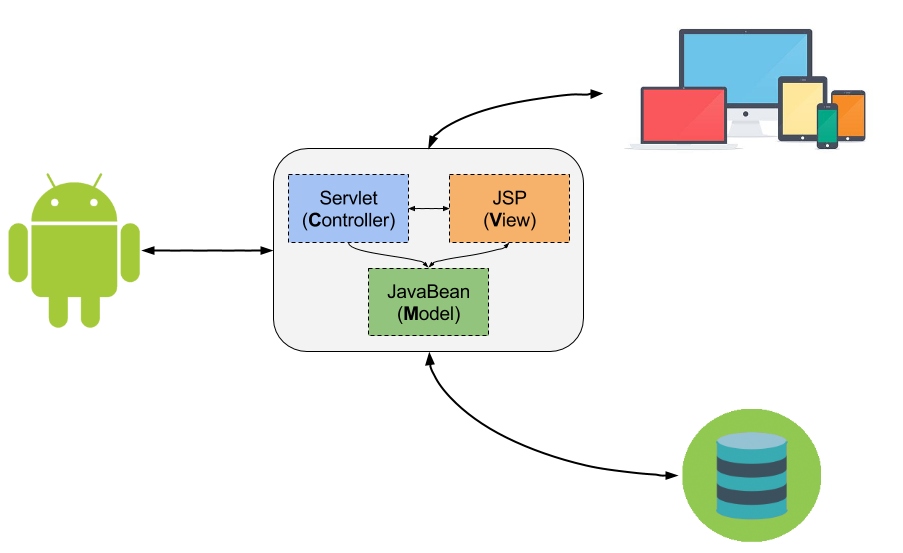
\includegraphics[width=1\textwidth]{StrukturaSystemu.png}
\caption{Schemat zaprojektowanego systemu lokalizacji przesyłek kurierskich}
\label{StrukturaSystemu}
\end{figure}

Zaprojektowaną aplikację zrealizowano w środowisku programistycznym Eclipse.
Wybór takie środowiska programistycznego uwarunkowany był dużym wyborem
dodatków, rozszerzeń i możliwości jaką on oferuje.

\newpage
\section{Aplikacja na system Android}

Założeniem aplikacji mobilnej było lokalizowanie kuriera i wysyłanie jego
pozycji na serwer, który zapisuje ją w bazie danych. Zasada działania aplikacji
polega na odpytaniu kuriera o jego numer id, a następnie sprawdzeniu czy jest
włączony GPS. Ponadto aplikacja wykrywa czy wprowadzono poprawne id oraz
zapobiega zalogowaniu się dwóch kurierów na tym samym id. Po wpisaniu poprawnego
id kuriera aplikacja zapamiętuje go i automatycznie wysyła swoją pozycję na serwer.

\begin{wrapfigure}{r}{0.4\textwidth}
\vspace{-25pt}
\centering
\captionsetup{justification=centering,margin=0cm}
\begin{center}
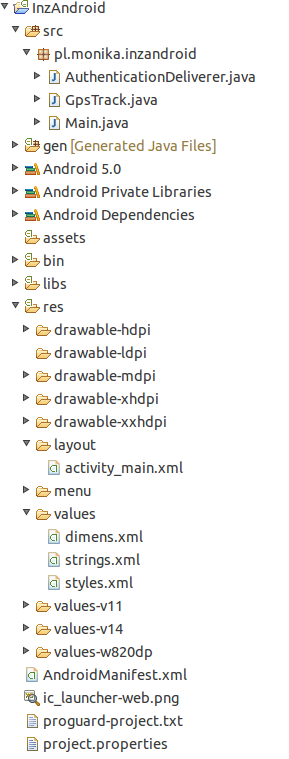
\includegraphics[width=.4\textwidth]{struktura_android.png}
\end{center}
\caption{Struktura plików programu aplikacji mobilnej w systemie Android}
\label{fig:androidStruktura}
\end{wrapfigure}

Projektowanie aplikacji na system Android zostało rozpoczęte od instalacji
pluginu ADT (Android Development Tools) dla programu Eclipse. W skład ADT
wchodzi między innymi Android SDK (Software Development Kit).
Android SDK zawiera w sobie takie elementy jak Tools -- służy do tworzenia aplikacji niezależnie od
wersji systemu Android oraz Platform Tools -- narzędzia stworzone pod kątem
wersji systemu Android. W skład SDK Tools wchodzą takie funkcje jak: zarządzanie
projektami, modułami czy maszynami wirtualnymi, debugger czy emulator,
Platform Tools natomiast zawiera biblioteki do systemu Android. Plugin ADT 
korzysta z funkcji Android SDK i pomaga tworzyć, budować, instalować oraz debugować
aplikacje na system Android w środowisku Eclipse. W programie Eclipse tworzona
jest wraz z aplikacją odpowiednia struktura projektu [rys. \ref{fig:androidStruktura}], w
której jest podział na klasy zawierające logikę aplikacji (src), pliki
generowane przez kompilator (gen), folder na pliki z zasobami (assets), pliki
binarne (bin), dodatkowe biblioteki (libs) oraz folder na zasoby (res), który
odróżnia od assets to, że znajdują się w nim zasoby generowane do pliku R.java
(nie trzeba podawać lokalizacji zasobu tylko jego nazwę). W katalogu projektu
ustalana również jest konfiguracja aplikacji -- ,,AndroidManifest.xml'', layout
(wygląd i ustawienie elementów na ekranie systemu Android), w podfolderach
drawable umieszcza się pliki graficzne, w podfolderach values ciągi znaków
(stringi, kolory i in.) i ustawienia, a w katalogu menu -- dostępne opcje menu.

Projektowanie aplikacji Android zaczyna się od ustawienia układu graficznego
(/res/layout/activity\_main.xml). Zaprojektowany przez autora układ graficzny jest
prosty i przejrzysty, ponieważ ma wykonywać bardzo podstawowe funkcje [rys.
\ref{fig:androidViewOK}]. I tak, zawiera w sobie pole do wpisywania id kuriera,
pole wyświetlające komunikaty oraz przycisk wyłączający aplikację. Aplikacja została
tak przemyślana, że aby ją wyłączyć trzeba użyć przycisku ,,Off'', pozostałe
sprzętowe przyciski nie wyłączają aplikacji, jedynie ją minimalizują. Takie
właściwości zostały stworzone z myślą o tym, aby kurier podczas używania aplikacji tylko w świadomy
sposób mógł ją zamknąć.

Autor przewidział również odpowiednie zachowanie aplikacji, gdy kurier próbuje
zalogować się na nieistniejące w bazie id lub na id, które jest już zajęte -
tzn. na które już zalogował się inny kurier [rys. \ref{fig:androidViewNOTOK}]. 
Oprócz wyżej wymienionych zachowań aplikacji, w pasku statusu na telefonie
wyświetlana jest ikona podczas włączonej aplikacji, a także w
powiadomieniach [rys. \ref{fig:androidViewtask}].

Kolejnym krokiem było nadanie odpowiednich uprawnień aplikacji, do czego służy
plik ,,AndroidManifest.xml''. Aplikacji zostały przyznane uprawnienia do
sprawdzania statusu sieci komórkowej oraz WiFi, sprawdzania statusu sygnału
GPS, a także do korzystania z wyżej wymienionych [listing \ref{lst:manifest}].

\lstset{language=XML,
 keywords=[0]{uses,permission},
 keywordstyle=[0]{\color{green!50!black}},
 stringstyle=\color{blue}
 }
\begin{lstlisting}[caption=Nadanie uprawnień aplikacji
Android w pliku AndroidManifest.xml,label=lst:manifest] 
<uses-permission android:name="android.permission.INTERNET" />
<uses-permission android:name="android.permission.ACCESS_NETWORK_STATE" />
<uses-permission android:name="android.permission.ACCESS_FINE_LOCATION" />
<uses-permission android:name="android.permission.ACCESS_WIFI_STATE" />
\end{lstlisting}

\begin{figure}
\centering
\captionsetup{justification=centering,margin=1cm}
\subfigure[]{\label{figa1}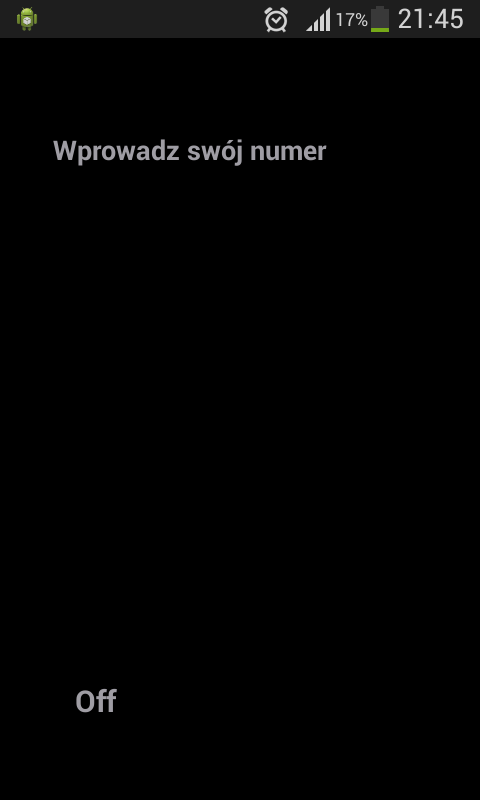
\includegraphics[height=0.35\textheight]{andWprowadz.png}}
\subfigure[]{\label{figa2}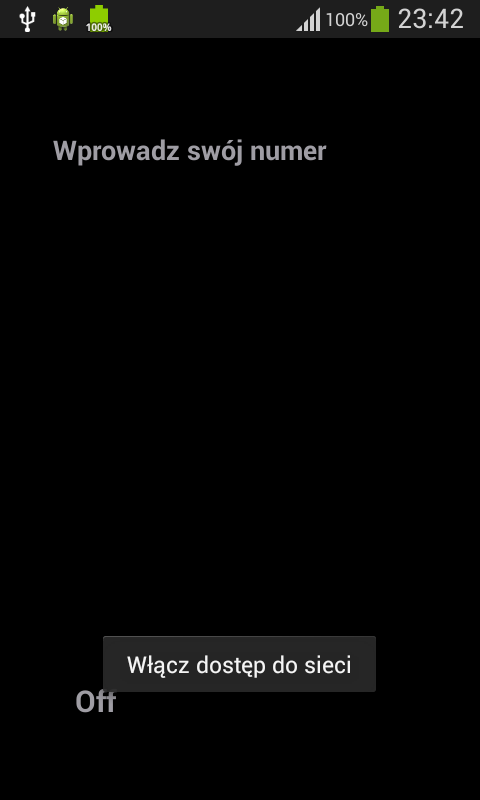
\includegraphics[height=0.35\textheight]{andWifi.png}}
\subfigure[]{\label{figa3}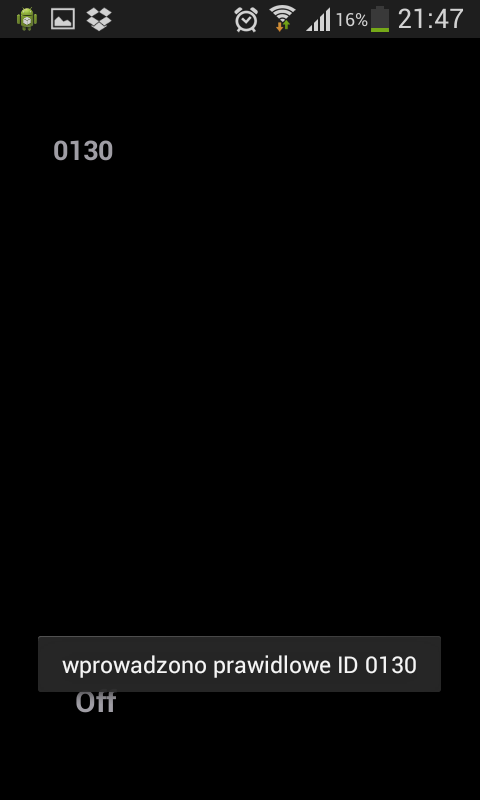
\includegraphics[height=0.35\textheight]{andID.png}}
\subfigure[]{\label{figa4}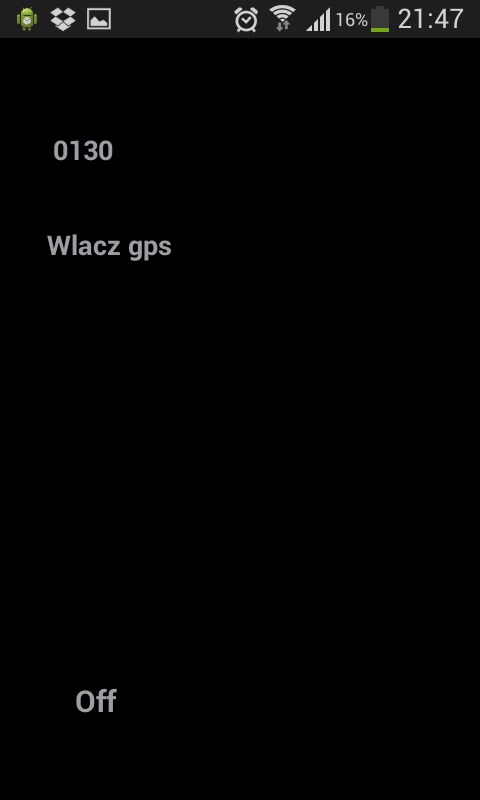
\includegraphics[height=0.35\textheight]{andGPS.png}}
\subfigure[]{\label{figa5}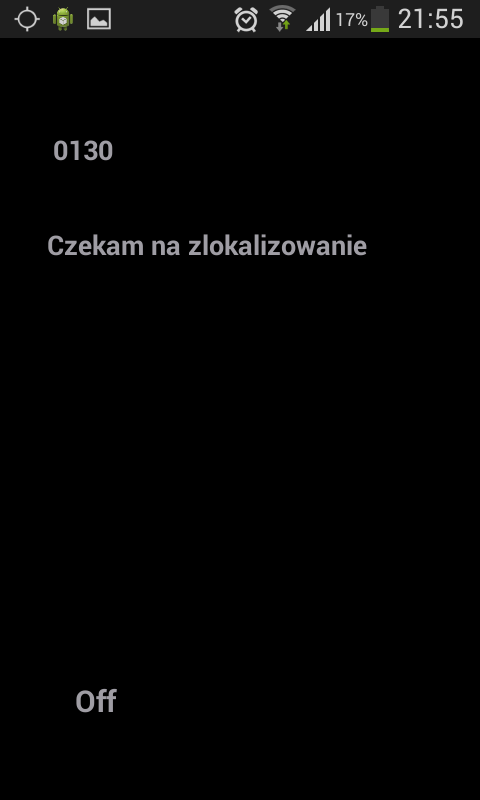
\includegraphics[height=0.35\textheight]{andCzeka.png}}
\subfigure[]{\label{figa6}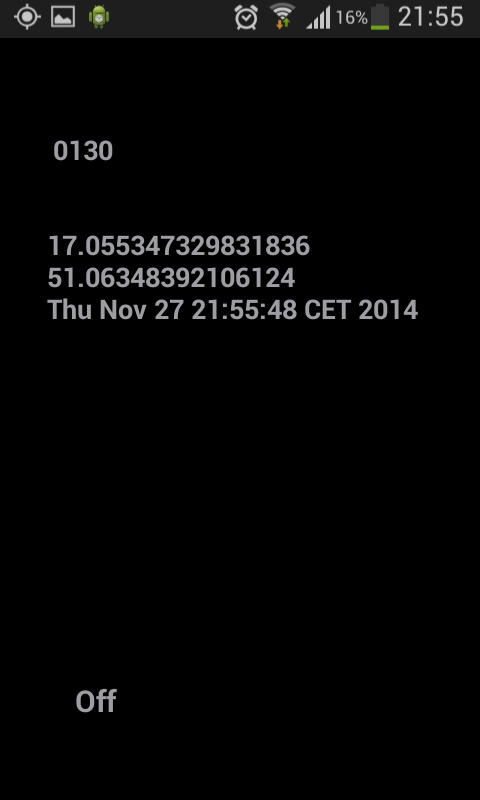
\includegraphics[height=0.35\textheight]{andLokal.png}}
\caption{Ekrany systemu Android: \subref{figa1} główny ekran
aplikacji, oczekuje na wprowadzenie id
kuriera; \subref{figa2} gdy nie jest włączona sieć komórkowa lub WiFi na
ekranie pokazuje się komunikat i zostaje zablokowane pole do wprowadzania
id; \subref{figa3} komunikat o poprawnie wpisanym id; \subref{figa4} informacje
o niewłączonym GPS; \subref{figa5} system czeka na ustalenie lokalizacji;
\subref{figa6} system lokalizuje i wyświetla informacje o lokalizacji i czasie
odczytu}
\label{fig:androidViewOK}
\end{figure}

Po przygotowaniu wyglądu aplikacji oraz nadaniu jej uprawnień można przejść
do oprogramowania logiki aplikacji. Klasa główna, która zajmuje się obsługą
aplikacji dziedziczy po klasie \texttt{Activity}. Klasa \texttt{Activity} zajmuje
się obsługą interakcji pomiędzy użytkownikiem a urządzeniem. Klasa ta tworzy okno aplikacji
oraz na przykład umieszcza ustawione wcześniej przyciski interfejsu użytkownika.
Znajdują się w niej takie metody jak \texttt{onCreate()}, \texttt{onDestroy()},
\texttt{onStart()}, \texttt{onStop()} i inne. Metodę \texttt{onCreate()} należy
przesłonić, jeśli mają być zainicjowane wcześniej wspomniane przyciski i pola z layoutu. Autor w swojej aplikacji nadaje taką
właściwość dla przycisku, która po kliknięciu go w dowolnym momencie
działania aplikacji wywołać zamknięcie jej. Takie zachowanie osiąga się
poprzez wywołanie na rzecz niego metody \texttt{public void
setOnClickListener(View.OnClickListener l)}[listing \ref{lst:Main.button.java}].

\lstset{language=Java,firstnumber=1,stepnumber=1,keywords=[3]{button,savedId}}
\begin{lstlisting}[caption=Ustawienie właściwości przycisku
``Off'' w głównej klasie aplikacji mobilnej w
metodzie onCreate(),label=lst:Main.button.java] 
button.setOnClickListener(new View.OnClickListener() { 
	public void onClick(View v) { 
		if (savedId != "")
			new AuthenticationDeliverer().execute(savedId, "0", "0").get();
		savedId = "";
		onDestroy();
	}
});
\end{lstlisting}
%%%%%%%%%%%%%%%%%%%%%%%%%%%%%%%%%%%%%%%%%%%%%%%%%%%%%%%%%%%%%%%%%%%%%%%%%%%%%%%%%%%%%%%%%%%%%%%%%%%%%%%%%%%%%%%%%%%%%%%%%%%%%%%%%%
%onDestroy na finish
%%%%%%%%%%%%%%%%%%%%%

Na listingu \ref{lst:Main.button.java} widać zmienną \texttt{savedId}. 
Jest to pole klasy, które zapisywane jest wprowadzonym przez kuriera jego \texttt{id}. Gdy użytkownik wyłącza
aplikację system sprawdza czy \texttt{savedId} nie jest puste i w przypadku gdy
\texttt{savedId} posiada jakąś wartość tworzony jest nowy obiekt
\texttt{AuthenticationDeliverer()} z odpowiednimi parametrami -- identyfikator kuriera,
 status aktywności oraz status logowania. Klasa
\texttt{AuthenticationDeliverer()} dziedziczy po \texttt{AsyncTask} (umożliwia
tworzenie nowego wątku i pozwala na wykonywanie operacji w tle). 

\begin{figure}
\centering
\captionsetup{justification=centering,margin=1cm}
\subfigure[Sytuacja, w której identyfikator jest już zajęty lub nie istnieje]{
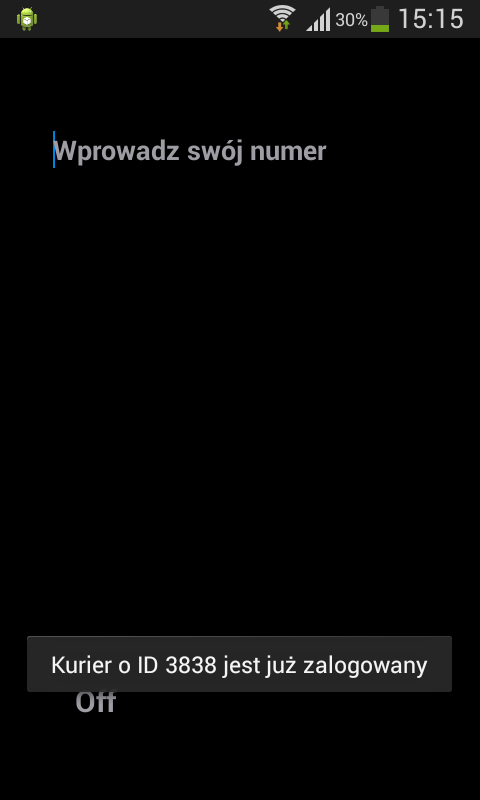
\includegraphics[height=0.35\textheight]{andJuzzalog.png}
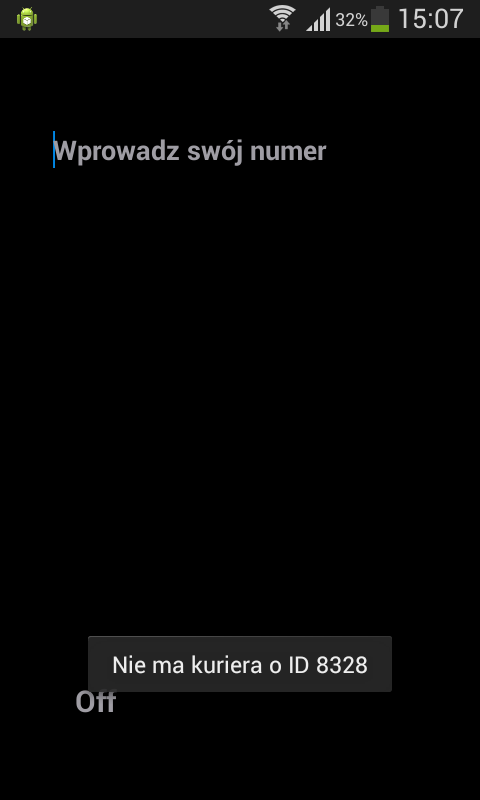
\includegraphics[height=0.35\textheight]{andNiema.png}
\label{fig:androidViewNOTOK}
}
\subfigure[Pasek status telefonu]{
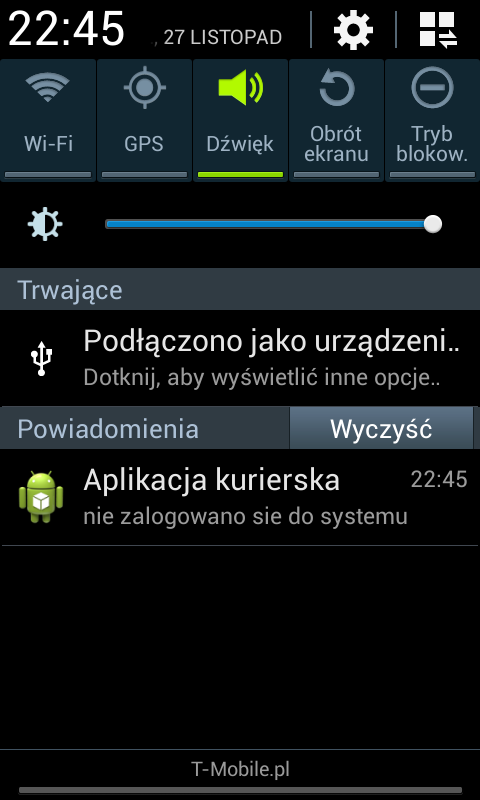
\includegraphics[height=0.35\textheight]{andBarNie.png}
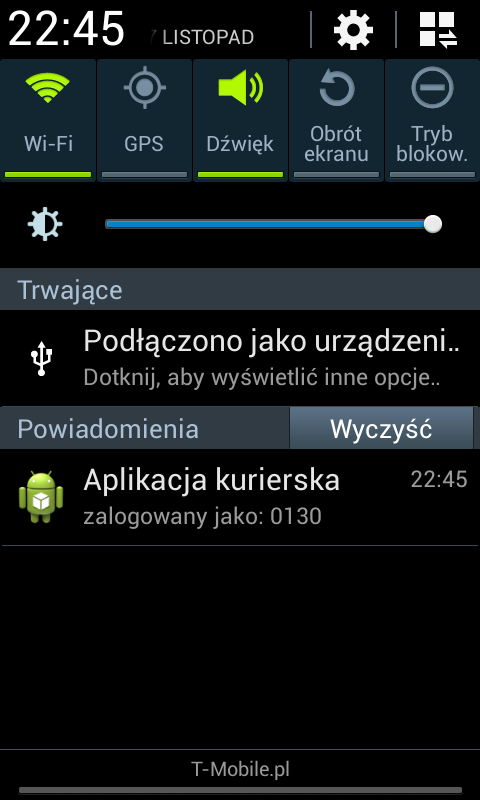
\includegraphics[height=0.35\textheight]{andBarZal.png}
\label{fig:androidViewtask}
}
\caption{Ekrany systemu Android: informacja o zalogowanym lub nieistniejącym
id oraz prezentacja uruchomionej aplikacji w pasku Statusbar}
\end{figure}

Parametry z jakimi tworzony jest
nowy obiekt to id kuriera, status aktywności oraz jego logowanie lub
wylogowywanie[listing. \ref{lst:AuthentictionDeliverer.java}]. Status aktywności to
informacja wysyłana do serwera (zapisywana w bazie danych) mówiąca o tym, czy kurier będzie ustawiał swój status na aktywny
czy nieaktywny -- czy rozpoczyna pracę czy ją kończy. Status aktywności
sprawdzany jest ze statusem w bazie danych, jeśli kurier próbuje się zalogować,
ale w bazie jest już ktoś zalogowany na ten id pojawi się komunikat o
zalogowanym już kurierze o tym numerze [rys. \ref{fig:androidViewNOTOK}].
Natomiast trzeci parametr mówi o tym, czy kurier się zalogowywuje (,,1'') czy
wylogowuje (,,0'') z aplikacji. Na rzecz klasy AuthenticationDeliverer()
wywołane zostają metody:
\texttt{execute()} -- nakazuje wykonanie zadania, \texttt{get()} -- oczekuje, aż
zadanie zostanie wykonane.

\lstset{language=Java,firstnumber=1,stepnumber=1,keywords=[3]{httpClient,localhost,
httpPostAuthentication,httpGetAuthentication,httpResponse}} 
\begin{lstlisting}[caption=klasa
AuthenticationDeliverer metoda
doInBackground,label=lst:AuthentictionDeliverer.java]
protected String doInBackground(String... params) {
	ArrayList<NameValuePair> pairs = new ArrayList<NameValuePair>();
	pairs.add(new BasicNameValuePair("ID", params[0]));
	pairs.add(new BasicNameValuePair("activ", params[1]));
	pairs.add(new BasicNameValuePair("logout", params[2]));
	httpPostAuthentication.setEntity(new UrlEncodedFormEntity(pairs));
	
	new Thread(new Runnable() {
		@Override
		public void run() {
				httpClient.execute(httpPostAuthentication);
		}
	}).start();
	
	httpResponse = (new DefaultHttpClient()).execute(httpGetAuthentication);
	String entityStr = EntityUtils.toString(httpResponse.getEntity());
	if (entityStr.contains("logIn"))
		return "logIn";
	else if (entityStr.contains("busy"))
		return "busy";
	else if (entityStr.contains("false"))
		return "false";
	else if (entityStr.contains("logOut"))
		return "logOut";
	return "";
}
\end{lstlisting}

Po zainicjalizowaniu pola edycji zostaje wywołana na rzecz niego metoda
\texttt{public void addTextChangedListener(TextWatcher watcher)}, która
oczekuje, aż w polu tekstowym użytkownik wpisze odpowiedni ciąg znaków -
dozwolone są tylko cyfry od 0 do 9. W tym przypadku wykorzystano metodę
\texttt{abstract void afterTextChanged(Editable s)} z interfejsu
\texttt{TextWatcher}. Po wpisaniu przez kuriera czterech cyfr następuje weryfikacja wpisanego id. Po pozytywnym
przejściu weryfikacji id kuriera aplikacja sprawdza czy w urządzeniu jest
włączony moduł GPS. Gdy spełnione zostaną wszystkie warunki uruchamiany jest
handler, który sczytuje pozycję kuriera i wysyła ją na serwer wraz z datą odczytu. 

Odczyt pozycji GPS dostępny jest dzięki użyciu klasy \texttt{LocationManager},
która zapewnia dostęp do systemowej usługi lokalizacji. \texttt{LocationManager}
należy zainicjalizować instancją klasy \texttt{Context} (umożliwia dostęp do
zasobów systemu i informacji o nim), natomiast \texttt{getSystemService} służy
do kontroli pobierania lokalizacji. Następnie ustawiono z jaką częstotliwością
ma być odczytywana zmiana pozycji. Po wykonaniu tych czynności następuje
zapytanie o ostatnią znaną pozycję. Całą procedurę odczytu pozycji GPS pokazano
na listingu \ref{lst:GpsTrack.java}.

\lstset{language=Java,firstnumber=1,stepnumber=1,keywords=[3]{locationManager,context,minTime,
minDistance,location,longitude,latitude}} 
\begin{lstlisting}[caption=Pobieranie lokalizacji
kuriera metoda getLocation() z klasy GpsTrack,label=lst:GpsTrack.java]
public Location getLocation() {
	locationManager = (LocationManager) context
			.getSystemService(Context.LOCATION_SERVICE);
	locationManager.requestLocationUpdates(LocationManager.GPS_PROVIDER,
			minTime, minDistance, (android.location.LocationListener) this);
			
	if (locationManager != null) {
		location = locationManager.getLastKnownLocation(LocationManager.GPS_PROVIDER);
		if (location != null) {
			longitude = location.getLongitude();
			latitude = location.getLatitude();
		}
	}
	return location;
}
\end{lstlisting}

Ostatnią istotną częścią jaka realizowana jest na systemie Android jest połączenie
z serwerem. Nim zostanie nawiązane połączenie konieczne jest przygotowanie
treści wiadomości jaka ma zostać wysłana na adres serwera. Następuje to poprzez
wpisanie par ciągów znaków do tablicy, z czego jedna jest kluczem -- identyfikatorem,
a druga to jego wartość. Na jej podstawie budowany jest URL i wykonywany do zapytania
 HTTP (tutaj na Servlecie) typu
\texttt{Get}. Taka wiadomość może wyglądać w tym przypadku tak:

\begin{flushright}
\texttt{http://192.168.1.2:8080/inzServlet/insert?ID=0130\&longitude=50.3545\&latitude=11.3483
\\$\hookrightarrow$\&timestamp=2014-11-25+15:14:55\&activ=1}
\end{flushright}

\lstset{language=Java,firstnumber=1,stepnumber=1,keywords=[3]{savedId,
httpClient, httpPost,localhost}}
\begin{lstlisting}[caption=Metoda startSendGpsDate() klasy
Main.java. Metoda sprawdza stan sygnału GPS i przygotowuje wiadomość do
wysłania na serwer oraz wysyła ją,label=lst:Main.startSendGpsDate.java]
private String localhost = "192.168.1.2:8080";
private HttpClient httpClient = new DefaultHttpClient();
private HttpPost httpPost = new HttpPost("http://" + localhost
		+ "/inzServlet/insert");
(*@\centerline{\raisebox{0pt}[0pt][0pt]{$\vdots$}}@*)
private void startSendGpsDate() {
	if (gpsTrack.isGpsEnable()) {
		gpsTrack.getLocation();
		double lat = gpsTrack.getLatitude();
		double lon = gpsTrack.getLongitude();
		if (lat != 0.0 && lon != 0.0) {
			Date date = new Date(System.currentTimeMillis());
			textView.setText(lon + "\n" + lat + "\n" + date);
			ArrayList<NameValuePair> pairs = new ArrayList<NameValuePair>();
			pairs.add(new BasicNameValuePair("ID", savedId));
			pairs.add(new BasicNameValuePair("longitude", lon + ""));
			pairs.add(new BasicNameValuePair("latitude", lat + ""));
			pairs.add(new BasicNameValuePair("timestamp",
					new SimpleDateFormat("yyyy-MM-dd HH:mm:ss").format(date)));
			pairs.add(new BasicNameValuePair("activ", 1 + ""));
			httpPost.setEntity(new UrlEncodedFormEntity(pairs));
			new Thread(new Runnable() {
				@Override
				public void run() {
					httpClient.execute(httpPost);
				}
			}).start();
		} else
			textView.setText("Czekam na zlokalizowanie");
	} else {
		textView.setText("Wlacz gps");
	}
}
\end{lstlisting}

W powyższym paragrafie zostały opisane kluczowe funkcje klas zaimplementowanych
w systemie Android. W opisie i w listingach pominięto obsługę wyjątków. 

\section{Serwer}

W niniejszej pracy skorzystano z możliwości rozszerzenie języka Java o funkcje
serwera WWW. Zadaniem Servletu (apletu Javy) było obsłużenie klientów firmy
kurierskiej, którzy wpisując numer swojej przesyłki mogli sprawdzić gdzie się
ona aktualnie znajduje. Oprócz tej funkcji Servlet też jest pośrednikiem
między aplikacją mobilną, a bazą danych.

\begin{wrapfigure}{r}{0.45\textwidth}
\centering
\captionsetup{justification=centering,margin=0cm}
\vspace{-10pt}
\begin{centering}
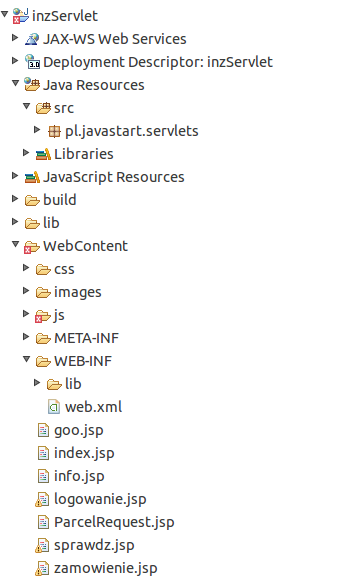
\includegraphics[width=.45\textwidth]{strukturaServlet.png}
\end{centering}
%\vspace{-10pt}
  \caption{Struktura plików programu Servletu}
\label{fig:servlet}
\vspace{-60pt}
\end{wrapfigure}

Rozpoczęcie pracy z Servletem wymagało zainstalowania dodatków do środowiska
Eclipse:
\begin{itemize}
  \item Eclipse Java EE Developer Tools
  \item Eclipse Java Web Developer Tools
  \item Eclipse Web Developer Tools
  \item JST Server Adapters
  \item JST Server Adapters Extensions
\end{itemize}

Po zainstalowaniu dodatków należało skonfigurować środowisko. W tym celu
należało stworzyć nowy lokalny serwer. Autor skorzystał z popularnego serwera Apache
Tomcat w wersji 7.0. Serwer nasłuchuje połączeń pod adresem localhost na
porcie 8080.

\makebox[\linewidth][s]{Po skonfigurowaniu środowiska można było }
\makebox[\linewidth][s]{przystąpić do utworzenia nowego dynamicznego}
\makebox[\linewidth][s]{projektu sieciowego (\texttt{Dynamic Web Project}).} 
\makebox[\linewidth][s]{W strukturze projektu najważniejsze są dwa}
\makebox[\linewidth][s]{foldery [rys. \ref{fig:servlet}]: pierwszy zawierający w
sobie} \makebox[\linewidth][s]{klasy Javy, oraz drugi
definiujący zachowanie i wygląd} \makebox[\linewidth][s]{stron Servletu.
W tymże folderze znajduje się} \makebox[\linewidth][s]{plik ,,web.xml'', w
którym definiuje się zachowanie} \makebox[\linewidth][s]{serwera w zależności od
tego jaki adres został} wpisany w przeglądarce.

Na poniższym listingu widać ustawienie strony startowej
(\texttt{<welcome-file-list>}). Gdy w polu adresy wpisany jest
\texttt{http://localhost:8080/inzServlet} uruchamia się strona główna aplikacji
webowej -- Index.jsp. W następnych liniach ładowana jest klasa
Javy (\texttt{pl.javastart.servlets.Sprawdz}) do Servletu pod nazwą
\texttt{Sprawdz} i następuje zmapowanie tej klasy pod adres
\texttt{http://localhost:8080/inzServlet/sprawdz}. Pokazany tu sposób dotyczy
wszystkich używanych przez Servlet klas. W podobny sposób można zadeklarować użycie
pliku *.jsp (różnica polega na zamianie identyfikatora \texttt{<servlet-class>}
na \texttt{<jsp-file>}). 

\lstset{language=XML,firstnumber=1,stepnumber=1}
\begin{lstlisting}[caption=Fragment pliku web.xml,label=lst:web.xml]
<welcome-file-list>
	<welcome-file>index.jsp</welcome-file>
</welcome-file-list>
<servlet>
	<servlet-name>Sprawdz</servlet-name>
	<servlet-class>pl.javastart.servlets.Sprawdz</servlet-class>
</servlet>
<servlet-mapping>
	<servlet-name>Sprawdz</servlet-name>
	<url-pattern>/sprawdz</url-pattern>
</servlet-mapping>
<servlet>
	<servlet-name>Index</servlet-name>
	<jsp-file>/index.jsp</jsp-file>
</servlet>
<servlet-mapping>
	<servlet-name>Index</servlet-name>
	<url-pattern>/index</url-pattern>
</servlet-mapping>
\end{lstlisting}

Każda klasa Javy, która rozszerza Servlet posiada dwie istotne metody do obsługi
stron serwera -- \texttt{doPost} i \texttt{doGet}. Obydwie przyjmują argumenty
typu \texttt{HttpServletRequest} i \texttt{HttpServletResponse}.
Metody mają zapewniać komunikację pomiędzy serwerem i klientem. Argument
\texttt{HttpServletRequest} zawiera żądanie klienta do wykonania na Servlecie,
natomiast \texttt{HttpServletResponse} jest odpowiedzią serwera na żądanie
klienta.
Wspomniana metoda \texttt{doGet} obsługuje żądania jakie zostały przesłane w
nagłówku HTTP -- pobiera parametry i przetwarza je. Metoda \texttt{doPost}
również obsługuje żądanie powstałe z uzupełnienia formularza.

Ważną klasą w projekcie jest klasa obsługująca bazę danych. Klasa do obsługi
bazy danych musi składać się z następujących poleceń: załadowanie sterownika
bazy danych, nawiązanie połączenia z bazą,
\makebox[\linewidth][s]{pobranie/zapisanie danych, zamknięcie połączenia.
Przykładem obsługi bazy danych jest poniższy}
\makebox[\linewidth][s]{listing [listing
\ref{lst:CheckIsExistsDeveliverer.selectFromDB.java}]. Przedstawiona metoda
sprawdza czy dany kurier istnieje w bazie. Sprawdzenie}
\makebox[\linewidth][s]{istnienia kuriera realizowane jest przez zapytanie
\texttt{"select * from deli.deliverer where id=" + id},} 
\makebox[\linewidth][s]{gdzie id jest
identyfikatorem kuriera. Po wykonaniu zapytania pod \texttt{ResultSet}
zapisywane są dane}
\makebox[\linewidth][s]{pobrane z bazy danych, z nich wyszukiwane są potrzebne
informacje, czyli id kuriera oraz} \makebox[\linewidth][s]{jego status
aktywności. \texttt{Id} pobierane jest tylko w celu sprawdzenia czy w bazie
istnieje kurier,} \makebox[\linewidth][s]{niestety nie ma metody dla
\texttt{ResultSet} która sprawdzałaby czy wynik zapytania jest pusty.} 
\makebox[\linewidth][s]{Po
uzyskaniu wyniku, że kurier istnieje sprawdzana jest
jego aktywność. Gdy kurier jest} 
\makebox[\linewidth][s]{nieaktywny a funkcja była wywoływana w celu
zalogowania do systemu przygotowywane jest} \makebox[\linewidth][s]{zapytanie o
zaktualizowanie danych dla tego kuriera i ustawieniu jego aktywności na stan
aktywny (\texttt{true}).} \makebox[\linewidth][s]{Natomiast gdy aktywność id
kuriera ma wartość logiczną \texttt{true}, a kurier chce się zalogować} (metoda
została wykonana dla zalogowania do systemu) metoda zwraca ciąg ,,busy'' -- informuje o zajętości id.
W momencie wylogowywania kuriera (kiedy \texttt{activ == true}) a
\texttt{logout} wynosi 0 -- to przygotowywana jest komenda aktualizująca bazę
danych i pod wskazaną krotkę o numerze id zapisywana jest wartość 0 dla
parametru \texttt{activ}.

\lstset{language=Java,firstnumber=1,stepnumber=1,keywords=[3]{id,activ,logout}}
\begin{lstlisting}[caption=Połączenia z bazą danych na przykładzie metody
sprawdzającej istnienie kuriera oraz jego stan
używanej przez aplikację
mobilną,label=lst:CheckIsExistsDeveliverer.selectFromDB.java]
Class.forName("com.mysql.jdbc.Driver");
Connection connection = DriverManager.getConnection(
		"jdbc:mysql://localhost:3306/deli", "root", "password");
Statement statement = connection.createStatement();
stringSelect = "select * from deli.deliverer where id=" + id;
ResultSet resultSet = statement.executeQuery(stringSelect);

while (resultSet.next()) {
	delivererId = resultSet.getInt("id");
	delivererActiv = resultSet.getBoolean("activ");
} 

if (delivererId > 0) {
	if (delivererActiv == false) {
		sqlInsert = " update deli.deliverer set activ=1 where id=" + id;
		statement.executeUpdate(sqlInsert);
		connection.close();
		statement.close();
		return "logIn";
	} else if (delivererActiv == true) {
		if (logout.equals("0")) {
			sqlInsert = " update deli.deliverer set activ=0 where id=" + id;
			statement.executeUpdate(sqlInsert);
			connection.close();
			statement.close();
			return "logOut";
		} else if (logout.equals("1")) {
			connection.close();
			statement.close();
			return "busy";
		}
	}
} else
	return "false";
\end{lstlisting}

Projekt dążył do stworzenia przyjaznego dla użytkownika
-- klienta widoku lokalizacji przesyłki. Do \makebox[\linewidth][s]{osiągnięcia
tego celu użyto zmodyfikowanego przez autora darmowego szablonu pobranego}
\makebox[\linewidth][s]{z internetu \cite{szablon}. W zakładce \texttt{SPRAWDZ
PRZESYLKE} wpisywany jest numer przesyłki jaką klient}
\makebox[\linewidth][s]{chce sprawdzić [rys.
\ref{fig:sprawdz}]. Wpisany ciąg znaków jest sprawdzany pod kątem poprawności.}
\makebox[\linewidth][s]{Sprawdzane jest czy ciąg w formularzu jest wartością
liczbową i czy istnieje taka przesyłka.} \makebox[\linewidth][s]{Gdy w bazie nie
istnieje przesyłka pojawia się odpowiedni komunikat informujący o
nieistniejącej} \makebox[\linewidth][s]{przesyłce [rys. \ref{fig:niema}]. Gdy
użytkownik wprowadzi poprawny numer przesyłki zostaną}
\makebox[\linewidth][s]{wyświetlone takie informacje jak:
nadawca, odbiorca, czas nadania i czas odbioru oraz}
\makebox[\linewidth][s]{ostatnio sczytane położenie przesyłki. Ponadto
wyświetlana jest mapa pokazująca jaką} \makebox[\linewidth][s]{trasę pokona
przesyłka -- znaczniki A -- B. Na mapie dodatkowo pokazany jest znacznik, który}
wyznacza pozycję kuriera z daną przesyłką -- znacznik ,,kurier''.

Istotną częścią projektu było zaprojektowanie strony, na
której klient może sprawdzać status swojej \makebox[\linewidth][s]{przesyłki.
Zrealizowane jest to poprzez utworzenie pliku *.jsp, i przypisanie jej adresu
URL.} Ogólny zarys pliku sprawdz.jsp jest pobrany z szablonu \cite{szablon}, autor zmienił jedynie ciało pliku. 

Z formularza [rys. \ref{fig:sprawdz}] pobierany jest numer poszukiwanej
przesyłki [listing \ref{lst:Sprawdz.jsp} linie
\ref{lst:sprawdz.jsp1}-\ref{lst:sprawdz.jsp2}], ustawiany jako post formularza
i przesyłany do klasy Servletu. W tej klasie po pobraniu danych z bazy danych
\makebox[\linewidth][s]{zwracane są wartości dotyczące istnienia przesyłki o
wskazanym id. Najpierw sprawdzane jest,} \makebox[\linewidth][s]{we fragmencie
kodu Javy w instrukcji warunkowej, czy przesyłka istnieje
(\texttt{isParcelExists}).} \makebox[\linewidth][s]{Gdy przesyłka nie zostanie
odnaleziona w bazie lub wpisany ciąg w formularzu jest niepoprawny}
\makebox[\linewidth][s]{wyświetlana jest wiadomość [listing
\ref{lst:Sprawdz.jsp} linia \ref{lst:sprawdz.jsp6}] dotycząca błędnego id. Natomiast gdy wpisany} 
id jest bezbłędny w tabeli zostają wypisane dane dotyczące przesyłki oraz mapa
[rys.
\ref{fig:pokaz}]. Linia
\ref{lst:sprawdz.jsp5} listingu \ref{lst:Sprawdz.jsp} jest miejscem użycia
JavaScript'owego kodu map Google. W danych wejściowych zmienna \texttt{msg}
oznacza wiadomość dotyczącą niepoprawnie wpisanego numeru przesyłki, lub jeśli
przesyłka została poprawnie wpisana, ale jej ostatnie położenie jest
zarejestrowane w centrali to w tabeli w wierszu
\makebox[\linewidth][s]{,,Ostatnie zarejestrowane położenie'' pojawia się
dodatkowa informacje o pobycie przesyłki} w centrali.

\lstset{language=Java,firstnumber=1,stepnumber=1,keywords=[4]{script,
div,section,
table,td,tr,h2,form,input,br},keywords=[5]{width,id,method,action,type,name,value,style}}
\begin{lstlisting}[caption=Ciało pliku JavaServlet Pages -
sprawdz.jsp,label=lst:Sprawdz.jsp] 
(*@\label{lst:sprawdz.jsp1}@*)<h2>Wpisz nr przesylki</h2> 
	<form id="formularz" method="post" action=""> 
	<input type="text" name="nr" /> <input type="submit" value="sprawdz" />
</form> (*@\label{lst:sprawdz.jsp2}@*)
(*@\hspace{4ex}{\raisebox{-1pt}[0pt][0pt]{$\vdots$}}@*)
(*@\label{lst:sprawdz.jsp3}@*)<%

if (request.getAttribute("isParcelExists") != null &&
		request.getAttribute("isParcelExists").equals(true)) {
		
%>
(*@\label{lst:sprawdz.jsp4}@*)<table style="width:100%">
	<tr>
		<td><% out.print("Numer przesylki"); %></td>
		<td>${id}</td>
	</tr>
	<tr>
		<td><% out.print("Nadawca"); %></td>
		<td>${regUserName}<br> ${regUserAddr} </td>
	</tr>
	<tr>
		<td><% out.print("Czas nadania"); %></td>
		<td>${timeSend}</td>
	</tr>
	<tr>
		<td><% out.print("Odbiorca"); %></td>
		<td>${userName}<br> ${userAddr} </td>
	</tr>
	<tr>
		<td><% out.print("Planowany czas"); %><br> <% out.print("dostarczenia"); %>
		</td>
		<td>${timeDelivery}</td>
	</tr>
	<tr>
		<td><% out.print("Ostatnie zarejestrowane"); %><br>
			<% out.print("polozenie"); %></td>
		<td>${lastTime}<br>${msg}</td>
	</tr>
</table>
(*@\hspace{4ex}{\raisebox{-1pt}[0pt][0pt]{$\vdots$}}@*)
(*@\label{lst:sprawdz.jsp5}@*)<div id="mapka"> </div>
(*@\hspace{4ex}{\raisebox{-1pt}[0pt][0pt]{$\vdots$}}@*)
<%

}
(*@\label{lst:sprawdz.jsp6}@*)else {

%>
(*@\label{lst:sprawdz.jsp7}@*)<br> ${msg} ${id}
<% 

}

%>
\end{lstlisting}

Ustawianie parametrów umieszczonych w \$\{\ldots\} zrealizowano
poprzez klasę rozszerzającą Servlet. \makebox[\linewidth][s]{Na listingu
\ref{lst:Sprawdz.doPost.java} przedstawiono metodę \texttt{doPost()} klasy
\texttt{Sprawdz.java}, która odpowiada za} \makebox[\linewidth][s]{uzupełnianie
pliku JSP \texttt{sprawdz.jsp} danymi dotyczącymi przesyłki, które są
wyświetlane} \makebox[\linewidth][s]{w widoku strony dla klienta. Klasa
\texttt{Sprawdz} tworzy nowy obiekt klasy \texttt{SearchParcel}}
\makebox[\linewidth][s]{wywołując ją z argumentem id przesyłki.
Obiekt klasy \texttt{SearchParcel} odczytuje bazę danych}
\makebox[\linewidth][s]{i przypisuje wartości zmiennym (listing \ref{lst:SearchParcel.selectFromDB.java}). Następnie sprawdzane
jest w instrukcji} \makebox[\linewidth][s]{warunkowej if czy taka przesyłka
istnieje i wprowadzone znaki są liczbą całkowitą. Jeśli}
\makebox[\linewidth][s]{nie istnieje to w zależności od tego jaki błąd wystąpił
przygotowywana jest wiadomość} \makebox[\linewidth][s]{zwrotna dotycząca tego
błędu. Jeżeli jednak przesyłka istnieje ustawiane są parametry}
\makebox[\linewidth][s]{zwrotne \texttt{req.setAttribute(``\ldots'',\ldots)}.
Warto zwrócić uwagę na to, że pierwszy argument}
\makebox[\linewidth][s]{\texttt{setAttribute} musi być zgodny z oczekiwaną nazwą
zmiennej w pliku JSP, w inny wypadku} 
nie zostanie przypisana wartość z klasy Javy do JSP. Na przykład argumenty z listingu \ref{lst:Sprawdz.jsp} z linii \ref{lst:sprawdz.jsp7} muszą się zgadzać argument z listingu
\ref{lst:Sprawdz.doPost.java} z linii \ref{lst:Sprawdz.doPost.java1}-\ref{lst:Sprawdz.doPost.java2}.

\lstset{language=Java,firstnumber=1,stepnumber=1,keywords=[3]{}} 
\begin{lstlisting}[caption=Fragment klasy Sprawdz.java\,
metoda doPost(),label=lst:Sprawdz.doPost.java]
protected void doPost(HttpServletRequest req, HttpServletResponse resp) {
	String id = req.getParameter("nr");
	boolean isParcelExists = false;
	RequestDispatcher view = req.getRequestDispatcher("/sprawdz.jsp");
	
	if (id != null && (Sth.isInteger(id)) == true) {
		SearchParcel searchParcel = new SearchParcel(Integer.parseInt(id));
		if (searchParcel.getIsParcelExists() == true) {
			isParcelExists = true;
			req.setAttribute("id", id);
			req.setAttribute("lat", searchParcel.getDelivererLatitude());
			req.setAttribute("lon", searchParcel.getDelivererLongitude());
			req.setAttribute("regUserName",	searchParcel.getRegisteredUserNameUser());
			req.setAttribute("regUserAddr",	searchParcel.getRegisteredUserStreetUser() +
					" " + searchParcel.getRegisteredUserCityUser() + " " +
					searchParcel.getRegisteredUserCityCodeUser()); 
			req.setAttribute("timeSend", searchParcel.getParcelSendTime()
					.substring(0, 16));
			req.setAttribute("userName", searchParcel.getParcelAddresseeName());
			req.setAttribute("userAddr", searchParcel.getParcelAddresseeStreet() + " " +
					searchParcel.getParcelAddresseeCity() + " "	+ 
					searchParcel.getParcelAddresseeCityCode());
			req.setAttribute("timeDelivery", searchParcel .getParcelDeliveryTime()
					.substring(0, 16)); 
			req.setAttribute("lastTime", searchParcel.getParcelTimePos()
					.substring(0, 16));
			if (searchParcel.getDelivererId() > 999000) {
				searchParcel.selectBase(searchParcel.getDelivererId());
				req.setAttribute("msg", "Przesylka w bazie: "
						+ searchParcel.getCentreNameCentre());
			}
		} else {
			(*@\label{lst:Sprawdz.doPost.java1}@*)req.setAttribute("msg", "Nie mamy
			przesylki w bazie o numerze: ");
			(*@\label{lst:Sprawdz.doPost.java2}@*)req.setAttribute("id", id); 
	}
	
	if (id == null || (Sth.isInteger(id)) == false)
		req.setAttribute("msg", "Prosze podac poprawny numer przesylki"); 
	req.setAttribute("isParcelExists", isParcelExists);
	req.removeAttribute("nr");
	view.forward(req, resp);
};
\end{lstlisting}

Na podstawie źródła \cite{developer.google.maps} autor utworzył kod,
który wyświetla mapę ze znacznikami -- markerami. Z danych metody post pobierane
są wartości lat i lon (szerokość i długość geograficzna) dla kuriera oraz wartości
\texttt{regUserAddr} i \texttt{userAddr} oznaczające adres nadawcy i odbiorcy. W
skrypcie tworzony jest nowy obiekt klasy \texttt{DirectionsRenderer}, który jest
odpowiedzialny za wypełnienie (renderowanie)
\makebox[\linewidth][s]{wyświetlanej mapy oraz tworzony jest nowy obiekt
\texttt{DirectionsService}, który wylicza trasę}
\makebox[\linewidth][s]{pomiędzy punktami.
Do obiektu \texttt{DirectionsRenderer} przypisywane jest umiejscowienie}
\makebox[\linewidth][s]{elementu w układzie strony przez pobranie jego id oraz
możliwe jest ustawienie parametrów} \makebox[\linewidth][s]{mapy.
Kolejnym krokiem jest utworzenie znacznika na pozycji kuriera i dodanie go do
mapy.} \makebox[\linewidth][s]{Ostatnim etapem jest wyliczenie trasy pomiędzy
dwoma punktami: adresem nadawcy} i adresem odbiorcy.

\lstset{language=Java,firstnumber=1,stepnumber=1,keywords=[4]{script,
div,section, table},morekeywords={var, function},keywords=[5]{id,src}}
\begin{lstlisting}[caption=Kod JavaScript'owy pobierający mapę z
serwera Google,label=lst:maps.JS] 
<script src="https://maps.googleapis.com/maps/api/js?v=3.exp"></script> 
<script>
	var lat = "${lat}";
	var lon = "${lon}";
	var start = "${regUserAddr}";
	var end = "${userAddr}";
	var directionsRenderer = new google.maps.DirectionsRenderer();
	var directionsService = new google.maps.DirectionsService();
	var map;

	function initialize() {
		map = new google.maps.Map(document.getElementById('mapka'));
		directionsRenderer.setMap(map);
		new google.maps.Marker({
			position : new google.maps.LatLng(lat, lon),
			map : map,
			title : "Kurier"
		});
		
		var directionsRequest = {
			origin : start,
			destination : end,
			travelMode : google.maps.TravelMode.DRIVING
		};
		
		directionsService.route(directionsRequest, function(directionsResult, directionsStatus) {
				if (directionsStatus == google.maps.DirectionsStatus.OK) {
					directionsRenderer.setDirections(directionsResult);
			}
		});
	}
	
	google.maps.event.addDomListener(window, 'load', initialize);
</script>
\end{lstlisting}

Klasa \texttt{Sprawdz.java} obsługująca \texttt{sprawdz.jsp} tworzy nowy obiekt
klasy \texttt{SearchParcel} i podbiera od \makebox[\linewidth][s]{niego
potrzebne dane do wyświetlenia na stronie i przesyła je metodą \texttt{doPost}.}
\makebox[\linewidth][s]{Klasa \texttt{SearchParcel.java} przedstawiona jest na
listingu \ref{lst:SearchParcel.selectFromDB.java}. Klasa otwiera połączenie}
\makebox[\linewidth][s]{z bazą danych, następnie wykonując zapytania SQL pobiera
dane dotyczące przesyłki,} \makebox[\linewidth][s]{a posiadając już id kuriera,
który przewozi tę przesyłkę, pobiera jego położenie oraz} informacje o nadawcy
(zarejestrowanym użytkowniku). Ostatnim krokiem jest zamknięcie połączenia z bazą danych.

\begin{figure}
\centering
\captionsetup{justification=centering,margin=1cm}
\subfigure[]{\label{fig:sprawdz}
\includegraphics[width=.92\textwidth]{sprawdz.png}}
\subfigure[]{\label{fig:pokaz}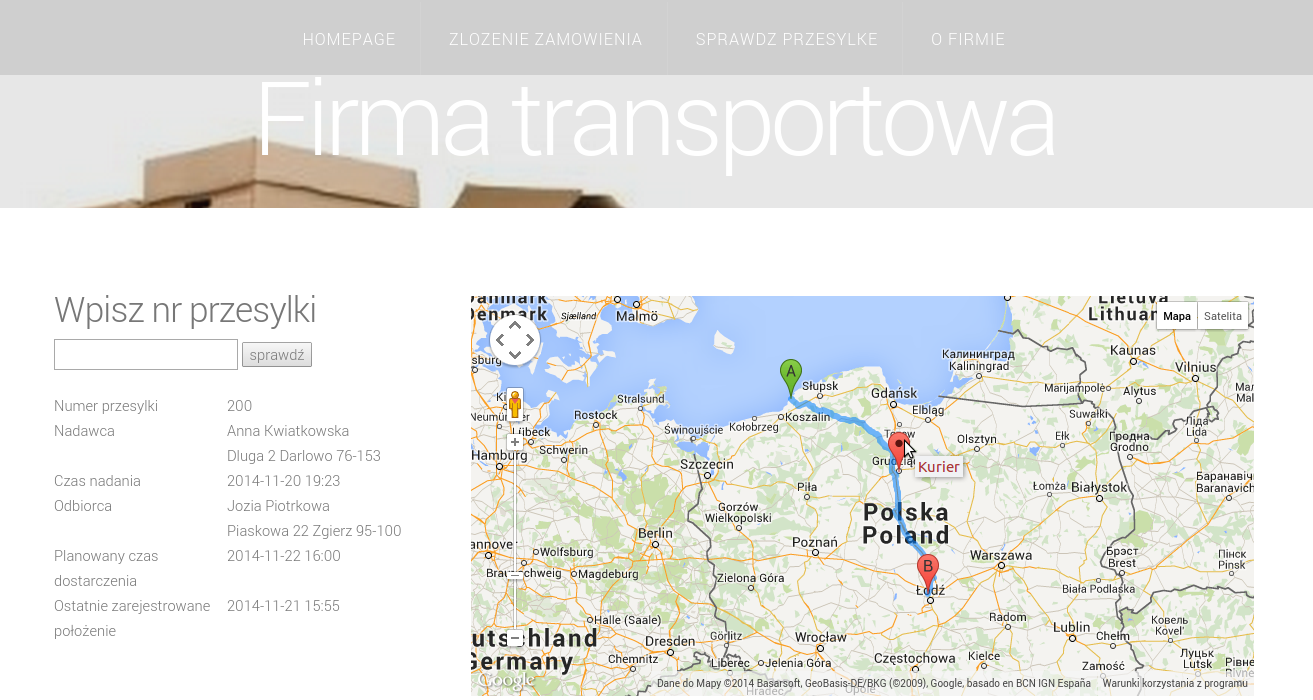
\includegraphics[width=.92\textwidth]{przyklad.png}}
\subfigure[]{\label{fig:niema}
\includegraphics[width=.92\textwidth]{nieMaPrzesylki.png}}
\caption{Okno aplikacji webowej i jego widoki: \subref{fig:sprawdz} widok strony
internetowej \texttt{SPRAWDZ} serwisu z zachętą do wprowadzenia numeru przesyłki do
sprawdzenia; \subref{fig:pokaz} widok strony internetowej \texttt{SPRAWDZ} z
wyznaczoną trasą dla przykładowej przesyłki; \subref{fig:niema} przykład
odpowiedzi serwisu na nieprawidłowe wpisanie numeru przesyłki}
\end{figure}

\lstset{language=Java,firstnumber=1,stepnumber=1,keywords=[3]{parcelId,
parcelFromUserId,parcelAddresseeName,parcelAddresseeStreet,
parcelAddresseeCity,parcelAddresseeCityCode,parcelSendTime,
parcelDeliveryTime,parcelDeliverer,isParcelExists,delivererId,
delivererLatitude,delivererLongitude,delivererTimePos,parcelFromUserId,
registeredUserId,registeredUserNameUser,registeredUserStreetUser,
registeredUserCityUser,registeredUserCityCodeUser,parcelTimePos}} 
\begin{lstlisting}[caption=Klasa SearchParcel.java przedstawiona metoda
selectFromDB()\, która reprezentuje połączenie z bazą danych oraz pobiera
wszystkie dane o przesyłce,label=lst:SearchParcel.selectFromDB.java]
public SearchParcel(int _nrParcel) {
	selectFromDB(_nrParcel); 
}

void selectFromDB(int nrParcel) {
	String strSelect = "";
	Class.forName("com.mysql.jdbc.Driver");
	Connection connection = DriverManager.getConnection(
			"jdbc:mysql://localhost:3306/deli", "root", "password");
	Statement statement = connection.createStatement();
	strSelect = "select * from deli.parcel where id=" + nrParcel;
	ResultSet resultSet = statement.executeQuery(strSelect);
	while (resultSet.next()) {
		isParcelExists = true;
		parcelId = resultSet.getInt("id");
		parcelFromUserId = resultSet.getInt("fromUserId");
		parcelAddresseeName = resultSet.getString("addresseeName");
		parcelAddresseeStreet = resultSet.getString("addresseeStreet");
		parcelAddresseeCity = resultSet.getString("addresseeCity");
		parcelAddresseeCityCode = resultSet
				.getString("addresseeCityCode");
		parcelSendTime = resultSet.getString("sendTime");
		parcelTimePos = resultSet.getString("timePos");
		parcelDeliveryTime = resultSet.getString("deliveryTime");
		parcelDeliverer = resultSet.getInt("deliverer");
	}
	if (isParcelExists == true) {
		strSelect = "select * from deli.deliverer where id="
				+ parcelDeliverer;
		resultSet = statement.executeQuery(strSelect);
		while (resultSet.next()) {
			delivererId = resultSet.getInt("id");
			delivererLatitude = resultSet.getDouble("latitude");
			delivererLongitude = resultSet.getDouble("longitude");
			delivererTimePos = resultSet.getString("timePos");
		}
		strSelect = "select * from deli.registeredUser where id="
				+ parcelFromUserId;
		resultSet = statement.executeQuery(strSelect);
		while (resultSet.next()) {
			registeredUserId = resultSet.getInt("id");
			registeredUserNameUser = resultSet
					.getString("nameUser");
			registeredUserStreetUser = resultSet
					.getString("streetUser");
			registeredUserCityUser = resultSet.getString("cityUser");
			registeredUserCityCodeUser = resultSet
					.getString("cityCodeUser");
		}
	}
	connection.close();
	statement.close();
}
\end{lstlisting}

Estymację czasu dostarczenia przesyłki zrealizowano
korzystając z usługi Google Distance \makebox[\linewidth][s]{Matrix API, z
której dostarczana jest odległość pomiędzy punktem nadania i odbioru}
\makebox[\linewidth][s]{przesyłki.
Wyznaczanie czasu dostarczenia wprowadzono równolegle z zapisem przesyłki}
\makebox[\linewidth][s]{do bazy danych. Autor nie mógł w inny sposób, niż
przedstawiony na listingu \ref{lst:wyliczCzasDostarczenia.DistanceMatrix.java},}
 tego wykonać z braku  próbek w postaci rzeczywistych danych. 

\lstset{language=Java,firstnumber=1,stepnumber=1,keywords=[3]{HOUR_OF_DAY,
czasPomiedzyDwomaPunktami,DAY_OF_MONTH}} 
\begin{lstlisting}[caption=Metoda
wyliczCzasDostarczenia() z
klasy DistanceMatrix,label=lst:wyliczCzasDostarczenia.DistanceMatrix.java]
public String wyliczCzasDostarczenia(Date sendTime) { 
	int days = 1;
	new SimpleDateFormat("yyyy-MM-dd HH:mm:ss")
			.format(new Date(czasPomiedzyDwomaPunktami * 1000L));
	Calendar calendar = GregorianCalendar.getInstance();
	calendar.setTime(sendTime);
	
	if (calendar.get(Calendar.HOUR_OF_DAY) > 18) {
		calendar.set(Calendar.HOUR_OF_DAY, 11);
		days++;
	}
	if (calendar.get(Calendar.HOUR_OF_DAY) > 0
			&& calendar.get(Calendar.HOUR_OF_DAY) < 12) {
		calendar.set(Calendar.HOUR_OF_DAY, 15);
	}
	if (czasPomiedzyDwomaPunktami < 1000) {
		days--;
	}
	if (czasPomiedzyDwomaPunktami > 20000) {
		days++;
	}
	calendar.add(Calendar.DAY_OF_MONTH, days);
	return new SimpleDateFormat("yyyy-MM-dd HH:mm:ss").format(calendar
			.getTime());
	}
\end{lstlisting}

Odległość i czas potrzebny do przebycia danej trasy uzyskano
formułując URL do zapytania \makebox[\linewidth][s]{serwisu Google Api
[listing \ref{lst:wyliczOdlegloscDistanceMatrix.DistanceMatrix.java}]. Z
uzyskanej odpowiedzi sprawdzono czy dana trasa istniej.} Gdy dane
wejściowe były poprawne status poszukiwanej trasy był \texttt{``OK''}, wtedy w zwrotnym
dokumencie podane były parametry drogi -- czas i odległość.

\lstset{language=Java,firstnumber=1,stepnumber=1,keywords=[3]{HOUR_OF_DAY,
czasPomiedzyDwomaPunktami,DAY_OF_MONTH,statusPomiedzyDwomaPuntmi,odlegloscPomiedzyDwomaPunktami}}
\begin{lstlisting}[caption=Metoda
wyliczOdlegloscDistanceMatrix() z
klasy
DistanceMatrix,label=lst:wyliczOdlegloscDistanceMatrix.DistanceMatrix.java] 
public Double wyliczOdlegloscDistanceMatrix(String ulNadania,
		String miastoNadania, String ulOdbioru, String miastoOdbioru) {
	String urlPath = "";
	urlPath = "http://maps.googleapis.com/maps/api/distancematrix/xml?origins="
			+ URLEncoder.encode(ulNadania, "UTF-8")
			+ "+"
			+ URLEncoder.encode(miastoNadania, "UTF-8")
			+ "&destinations="
			+ URLEncoder.encode(ulOdbioru, "UTF-8")
			+ "+"
			+ URLEncoder.encode(miastoOdbioru, "UTF-8")
			+ "&mode=driving&language=pl-PL&sensor=false";	
	Document document = null;
	document = DocumentBuilderFactory.newInstance()
			.newDocumentBuilder().parse(new URL(urlPath).openStream());	
	String str = toString(document);
	String tmp = str.substring(str.indexOf("status>") + "status>".length(),
			str.indexOf("</status"));

	if (tmp.equals("OK")) {
		statusPomiedzyDwomaPuntmi = true;
		odlegloscPomiedzyDwomaPunktami = Double.parseDouble(str.substring(
				str.indexOf("distance>") + 21, str.lastIndexOf("</val")));
		czasPomiedzyDwomaPunktami = Integer.parseInt(str.substring(
				str.indexOf("duration>") + 21, str.indexOf("</val")));
	} else
		statusPomiedzyDwomaPuntmi = false;
	return 0.0;
}
\end{lstlisting}

W podrozdziale Servlet nie pokazano obsługi wyjątków, a przedstawione listingi
są kluczowe do zrozumienia działania Servletu. Układ graficzny aplikacji webowej
został pobrany ze strony z darmowymi szablonami
{\textit{http://templated.co/linear}}.

\newpage
\section{Baza danych}

W przedstawionym projekcie konieczne było utworzenie bazy danych, która
przechowuje dane dotyczące kurierów, przesyłek, klientów, centrali kurierskich.
W tym celu stworzono cztery tabele: \texttt{parcel}, \texttt{deliverer},
\texttt{registeredUser} i \texttt{centre}.

\begin{figure}[ht!]
\centering
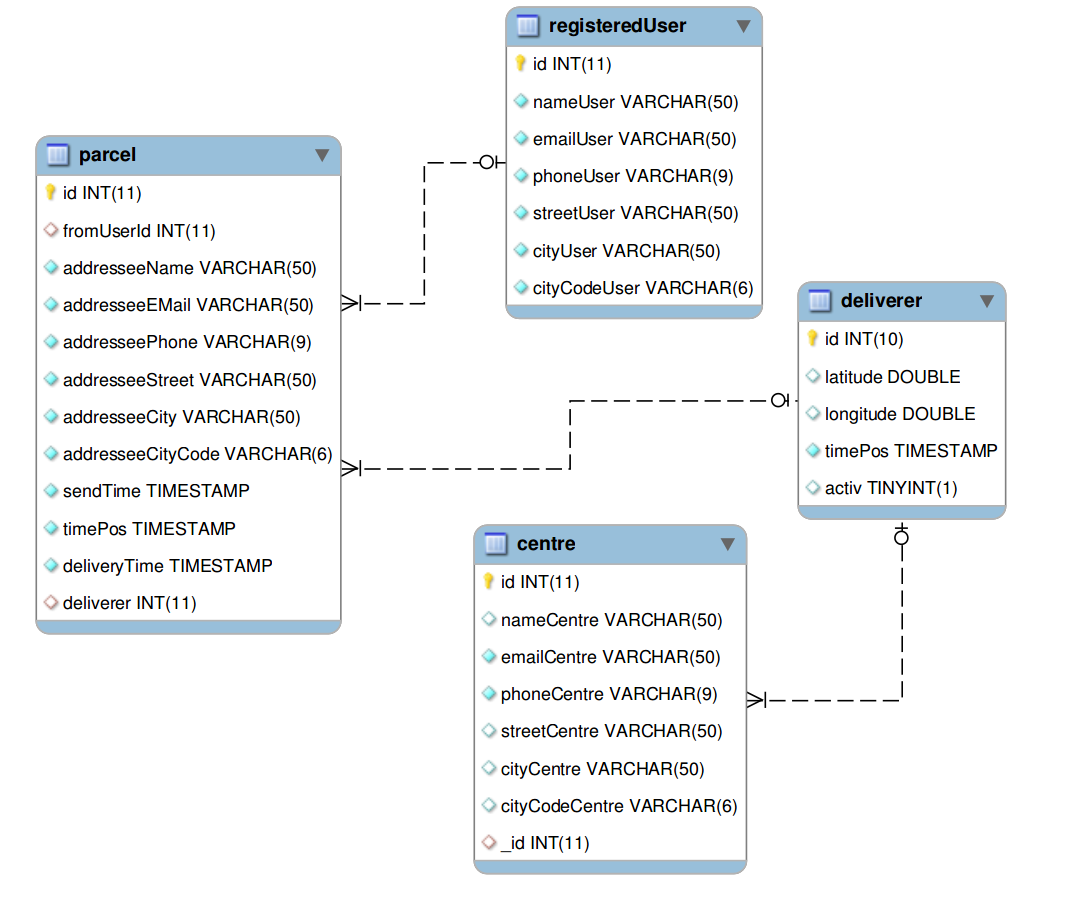
\includegraphics[width=0.9\textwidth]{ERD.png}
\caption{Diagram ERD zaprojektowanej bazy danych}
\label{fig:ERD}
\end{figure}

Na rysunku \ref{fig:ERD} przedstawiono diagram ERD pokazujący tabele oraz
połączenia pomiędzy nimi. Każda z tabel ma swój klucz główny (\texttt{id}).
Tabela \texttt{parcel} (przesyłka) zawiera w sobie dwa klucze obce
(\texttt{foreign key}) odwołujące się do \texttt{deliverer.id} -- klucza głównego
tabeli zawierającej informacje o kurierach oraz \texttt{registeredUser.id} -
klucz główny do tabeli użytkownika zarejestrowanego, czyli tego który złożył
zamówienie na dostarczenie przesyłki. Tabela \texttt{centre}, która ma zawierać
wpisy dotyczące nazwy, ulicy oraz miasta zawiera w sobie klucz obcy do tabeli
\texttt{deliverer}. Wybrano takie rozwiązanie ponieważ w tabeli
\texttt{deliverer} są podawane długość i szerokość geograficzna, które w łatwy sposób powiązano z tabelą \texttt{centre}.

\chapter{Przygotowanie i uruchomienie aplikacji}

Aby utworzyć opisywany w tej pracy projekt należy zacząć od instalacji IDE
Eclipse. Najprościej jest zacząć od instalacji Eclipse ADT z dodatkiem Android
SDK \cite{eclipse}, po jego instalacji w widoku Eclipse pojawi się ikona
,,Android SDK Manager''. Po załadowaniu się menedżera należy wybrać przynajmniej
SDK Tools, SDK Platform-tools, SDK Build-tools (najwyższą dostępną wersję), oraz w folderze z ostatnią wersją systemu Android X.X zaznaczyć SDK Platform i
obraz emulatora systemu Android (ARM EABI v7a System Image). Ponadto na
potrzeby tego projektu konieczne jest zainstalowanie Google Repository i Google
Play Services z folderu Extras.

Następnym krokiem jest zainstalowanie serwera Apache Tomcat w IDE Eclipse.
Dodanie nowego serwera rozpoczyna się od otworzenia zakładki
\texttt{Window>Preferences>Server>Runtine Enviroment}, gdzie należy dodać
(\texttt{add}) Apache Tomcat również w najnowszej wersji. Spowoduje to
dodanie serwera do bieżącej konfiguracji IDE.

Autor korzysta z systemu operacyjnego Linux (dystrybucja Ubuntu), więc zostanie
opisana instalacja silnika bazy danych w tym systemie. Do zainstalowania silnika
baz danych należy otworzyć okno terminalu, w którym trzeba wpisać komendę:

\texttt{sudo apt-get install mysql-server mysql-client} 
\newline Następnie należy postępować zgodnie z poleceniami instalatora,
użytkownik zobowiązany będzie do wpisana hasła dla użytkownika root. Po instalacji
silnik powinien zostać od razu uruchomiony, w celu sprawdzenia czy baza się
uruchomiła można wykonać komendę:

\texttt{sudo netstat -tap | grep mysql}
\newline lub

\texttt{sudo service mysql status}
\newline W razie konieczności uruchomienia (\texttt{start}), zastopowania
(\texttt{stop}) lub zrestartowania (\texttt{restart}) silnika bazy można użyć
odpowiednią komendę, np:

\texttt{sudo service mysql start}

Gdy w systemie zainstalowana już będzie baza to następnym krokiem jest
zainstalowanie wtyczki w IDE Eclipse. W menu \texttt{Help>Install New Software},
gdzie należy dodać (\texttt{Add}) nowe miejsce, z którego mają być ściągane
wtyczki dla danej wersji Eclipse i stamtąd pobierana będzie wtyczka ,,SQL Explorer''.
Przykładowo wersja, z której korzystał autor to:

\texttt{Juno - http://download.eclipse.org/releases/juno}

Jeśli w środowisku deweloperskim nie ma dodanych odpowiednich perspektyw,
należy je dodać (Open Perspective). Przydatne będą perspektywy
,,Java'' oraz ,,SQL Explorer''.
Po spełnieniu wszystkich wymienionych kroków można zaimportować
projekty. Import projektów odbywa się poprzez wybranie
\texttt{Import>Existing Project Into Workspace} z menu \texttt{File}.

\chapter{Wnioski i podsumowanie}


Aplikację można „podpiąć” pod prawdziwe urządzenia jakie posiadają kurierzy – te
na których się człowiek podpisuje – ale konieczne będzie
zrefakturyzowanie(?)/zmianie kodu pod system, który mają tam zainstalowany.
	Fajnie by było to wrzucić na prawdziwe tablety, można by sprzedawać/zarobić.
	Ogólnie koszt takiego urządzenia to byłoby tablet/telefon + wycena za program.
	Normalnie kurierzy używają kolektorów danych.
	
	
 Nie tylko GPS do lokalizacji, bo także odbicia
na czytnikach u kurierów Projekt opiera się 

Projekt został zrealizowany z wykorzystaniem takich
technologi jak: język programowania Java, system operacyjny Android, baza danych
MySQL, Google Apis. Firmy kurierskie maja najprawdopodobniej system „Windows
ce/mobile” na swoich urządzenia. Ja ze względu na brak takiego urządzenia
(mobilnego z Windowsem) zrealizuje zadanie na Androidzie.



Wykorzystanie rozwiązań bazujących na otwartym kodzie źródłowym w połączeniu 
z tanimi w eksploatacji i zakupie platformami sprzętowymi działającymi na systemie 
Android może stanowić ciekawą alternatywę dla firm przewozowych chcących wykorzystać 
funkcjonalną przewagę nad konkurencją jaką daje wizualizacja położenia przesyłki 
w czasie pseudorzeczywistym. Obecnie stosowane rozwiązania są mało dokładne, 
potrzebna infrastruktura jest droga, a konieczność stosowania aplikacji i 
platform bez publicznego API ogranicza możliwość rozbudowy.

Wszystkie wykorzystane w projekcie technologie mogą z powodzeniem zostać wykorzystane
 w projekcie komercyjnym. Wykorzystując fakt, że każdy dostawca musi zostać obowiązkowo
  wyposażony w telefon komórkowy można w prosty sposób zrealizować implementację
   opracowanego systemu bez dodatkowych nakładów finansowych na nowe urządzenia
    mobilne. Ponadto wykorzystanie publicznego API do komunikacji urządzeń z
     serwerem powoduje, że nie ogranicza nas system operacyjny urządzenia
      przenośnego (pod warunkiem, że na inny system również zostanie napisana 
      odpowiednia wersja aplikacji). Wykorzystanie publicznego interfejsu narzuca 
      jednak konieczność zadbania o bezpieczeństwo i spójność informacji, czyli, 
      np. autoryzację urządzenia przy zapytaniu czy wprowadzenie bezpiecznych połączeń https.

\ref{}

\addcontentsline{toc}{chapter}{Bibliografia} %utworzenie w spisie tresci pozycji Bibliografia
\bibliography{bibliografia} % wstawia bibliografie korzystajac z
% pliku bibliografia.bib -- dotyczy BibTeXa, jezeli nie korzystamy z BibTeXa nalezy uzyc otoczenia thebibliography

%opcjonalnie moze sie tu pojawic spis rysunkow i tabel
\listoffigures
\lstlistoflistings
\end{document}
